\documentclass[../tesi.tex]{subfiles}
\graphicspath{{../}}

%\usepackage[english]{babel}
\selectlanguage{english}%

\begin{document}
\chapter{Scientific Background and Related Work}
\begin{quotation}
\emph{qui va il cappello introduttivo, direi che lo aggiungo alla fine che ho descritto tutti gli argomenti dei related. }
\end{quotation}

\section{Physically Unclonable Function}
\puf{} are a physical entity designed to be easy to evaluate but hard to predict which uniquely identify a physical component.
\puf{} were first time presented in 2001 by Pappu \emph{et al.} namely Physical One-Way Functions (POWFs) in ~\cite{pappu2002physical} and ~\cite{ravikanth2001physical}. 
Usually, a malicious entity tries to steal information by mean of a physical attack to retrieve sensitive information from RAM or ROM, or more generally on a memory chip. 
Secure Storing of digital information from physical attacks is difficult and expensive where safe solutions are expensive. 
% Tenere questa frase magari per dopo. 
%Using a \tpm{} (\ref{sec:TPM}) could present lacks: decrypted secondary keys can be read out from the bus. \\
PUF is suitable to realize a low-cost solution for ICs authentication ~\cite{suh2007physical} while it can generate a secret volatile keys for cryptographic operations without store them. 
\puf{} outputs persistent and unpredictable results, called \emph{responses} , without the possibility to discover the input applied as a one-way function, namely \emph{challenges}.   
It is possible to define \emph{Challenge-Response Pairs (CRPs}): an unique set of couples for each device that contains a \puf{}. These can be implemented with several physical systems. In this thesis, we focus to Silicon \puf{s}, introduced by Gassend \emph{et al.} in  ~\cite{suh2007physical} and ~\cite{gassend2002silicon}. \\
These and other works offer a way for improving security in a system with a low costs ~\cite{guajardo2007fpga}. 
\begin{figure}
\centering
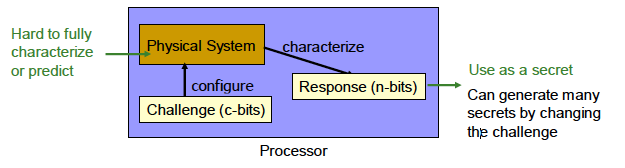
\includegraphics[scale=0.65]{images/firstpuf.png}
\caption{A logical PUF example}
\label{nome}
\end{figure}
The physical phenomena which mainly characterize \puf{} are the random variation in dies across a wafer, and from a wafer to wafer due to, i.e. process temperature and pressure variation, during the various manufacturing steps ~\cite{lofstrom2000ic}. Even a small variation in these variables door two chips to be different. 
Silicon \puf{s} have an exponential number of possible pair between challenges and response such that it is not possible to realize a software cloning of all the possible CRPs. 
\puf{s} can be realized for both Programmable Field Gate Arrays (FPGAs) and Application Specific Integrated Circuits (ASICs). 
\puf{'s} output looks like a random function that is unpredictable even for an attacker with physical access, this happen because, due to process variations, two integrated circuits are not identical ~\cite{suh2007physical}.
\subsection{PUF Properties}
Considering \puf{} as a mathematical function 
\begin{equation}
\prod : X  \rightarrow Y : \prod(x) = y 
\end{equation}
It is possible to highlight the relationship between challenge and response and present the following properties as described in ~\cite{maes2010physically} and ~\cite{gassend2002silicon}:
\begin{itemize}
\item \textbf{evaluable:} given $ \prod $ and $x$, y can be evaluate within polynomial time;
\item \textbf{unique:} $\prod$ can uniquely identify a device that embedds $\prod$.
\item \textbf{reproducible:} $y=\prod(x)$ is reproducible up to a small error\footnote{For this reason, \emph{reproducibility}, that \puf{} is different from TRNG (True Random Number Generator)}. 
\item \textbf{unclonable:} $\prod$ must be:
\begin{itemize}
\item \textit{physical unclonable}: it must be difficult to build a device containing another PUF $ \prod_{2}\neq \prod $ such that $ \prod_{2}(x) \approx \prod(x), \forall x; $
\item \textit{mathematically unclonable}: it must be difficult to build a mathematical function $f_{r}$ such that $f_{r} \approx \prod(x), \forall x;$
\end{itemize}
\item \textbf{unpredictable}: given only a Challenge Response Pair $\Phi=\lbrace(x_{i},y_{i}=\prod(x_{i}))\rbrace$ it is hard to predict value  $y_{c} \approx \prod x_{c}$ up to a small error, $\forall x_{c}$ being a random challenge do not exist $\Phi$;
\item \textbf{one-way}: given $y and \prod$ is difficult to find $x$ such that $\prod(x) = y$;
\item \textbf{tamper-evident}: if a malicious entity try to alter the device containing the function $\prod$ he obtain $\prod'$ with the transformation $ \prod \longrightarrow \prod' $ but $\prod(x) \neq \prod'(x), \forall x $. 
\end{itemize}
\subsection{Quality Metrics}  \label{par:qualitymetrics}
\puf{} validity can be estimated verifying that it produces responses respecting specific evaluation parameter, for this reason, the following quality metrics are presented, introduced by Maiti \emph{et al} in ~\cite{maiti2011improved}:
\begin{itemize}
\item \textbf{Uniqueness}: This factor estimates how PUF responses can distinguish chips each other. The Hamming Distance (HD) is the difference of bits between two bits string. Uniqueness is estimated using hamming distance between all the CPRs extracted from different devices. Uniqueness mathematical relationship is shown below:
\begin{equation}
U = \frac{2}{k(k-1)} \sum^{k-1}_{i=1} \sum^{k}_{j=i+1} \frac{HD(R_{i},R_{j})}{n} \cdot 100\%
\end{equation} 
K indicates the chips that implementing the same PUF design, each pair (i,j) of chips have a n-bit response $R_{i}$ and $R_{j}$ respectively. The ideal value of U is $50\%$.
\item \textbf{Reliability}: This factor gives an estimation about how is stable a PUF response under environmental changing, i.e. temperature or supply voltage. It specifically indicates the number of bits that change their value using the same challenge as input under different environmental conditions. It is called \emph{robustess }or \emph{intra-PUF variation}. Let $R_{i}$ be the n-bit baseline reference of the PUF with a specific design P, and k the number of generated measurements $R'_{i,j} (j=1,2,..k) $. The reliability can be defined as:
\begin{equation}
HD_{intra} = \frac{1}{k} \sum^{k}_{j=1} \frac{HD(R_{i},R'_{i,j})}{n} \cdot 100
\end{equation}
\begin{equation}
Reliability = 100 - HD_{intra}
\end{equation}
Reliability is the opposite of \emph{intra-chip Hamming Distance} and its ideal value is $100\%$. 
\item \textbf{Security/Attack Resilency}: PUF ability to prevent stealing of secrets to an adversary, like PUF CRPs.
\item \textbf{Uniformity}: This metric represents the distribution of 0 and 1 in the PUF response or in a PUFs sets of responses and can be mathematical described as:
\begin{equation}
RU(i) = \frac{1}{n} \sum^{n}_{t=1} R_{i,t} \cdot 100
\end{equation}
The variable, named \emph{n} is the number of response bits while \emph{i} is the i-th response. and can be correctly defined in percentage: $100\%$ means that all $R_{i}$ are 1.  A true random bits is characterized by an uniformity close as possible $50\%$. Let R be the number of considered response,\emph{RU} is the \emph{average uniformity}, represented as:
\begin{equation}
RU = \frac{1}{R} \sum^{R}_{i=1} RU(i)
\end{equation}
\item \textbf{Bit-Aliasing (BA) }: indicates that some response bits are biased towards either 0 or 1 on all devices. It can be defined as:
\begin{equation}
BA(t) = \frac{1}{k} \sum^{k}_{i=1} R_{i,t} \cdot 100
\end{equation}
where the variable \emph{t} indicates the t-th response bit, while \emph{k} is the number of devices. $R_{i,t}$ is the t-th response bit of the i-th device. If the result of this function is $100\%$ the t-th response bit is 1 for all the devices which execute the PUF. The ideal value is $50\%$. There is a strong relationship between uniformity and bit-aliasing, conversely, it is important to notice that even if BA of each response is around $50\%$ does not mean that bits are independent. On the other hand, independent bits can  lead to an uniformity percentage of $50\%$. 
\end{itemize}
\subsection{Use of PUF as Cryptographic Key} \label{fuzzyextractor}
Silicon \puf{} are characterized by noise responses due to circuit delays sensitive to environmental variations. In ~\cite{tuyls2006read} is noticed that \puf{} can be used as cryptographic key, hence, for \puf{} responses that are not fully random. Thus, in order to extract keys suitable for cryptographic approaches ~\cite{bosch2008efficient} post-processing techniques, as majority voting of fuzzy extraction approaches is required have been presented in literature.
Post-processing techniques allow to produce binary strings, eligible for cryptographic operations, from un-stable \puf{} responses. Majority voting is a post-processing technique based on multiple measurements over a \puf{} circuit \cite{maes2010intrinsic}. The measurement repetition can be done by averaging N sequential measurements on a PUF, using the Temporal Majority Voting (TMV) technique, or conversely, averaging N simultaneous measurements on different \puf{s} executing the Spatial Majority Voting (SMV).
Both TMV abd SMV evaluate different measurements in order to average extracted values and decide for the most frequent. Hence, such values need to be compared with pre-defined thresholds to establish the result of the voting. For this reason, majority could be not reliable in the case of average values near thresholds. 
Conversely, the fuzzy extractor technique involves only one measurement and exploits an error correction code (ECC) in order to retrieve stable binary strings from noisy responses.
A formal definition of fuzzy extractor is provided in ~\cite{dodis2004fuzzy} and ~\cite{linnartz2003new}. % Discorso più approfondito sull'argomento?  
Fuzzy extractor is composed of two basic primitives :
\begin{enumerate}
\item \textbf{Information Reconciliation (or Error Correction)}: which removes the error generated by the noise. This phase requires the adoption of error correcting codes %poi dopo, quando affronto la parte più implementativa casomai spiego bene Reed Muller e BCH!!
 \cite{gardner2009detecting} \cite{li2011viper} \cite{seshadri2005pioneer}, to correct bit errors in the PUF output obtaining a stable response.
% Questo concetto lo metto nell'appendice??
% The probability that a string with S bits will have more than t error is:
%\begin{equation}
%P_{total} =  1 - \sum^{t}_{i=0} \binom{S}{i} p_{b}^{i} (1-p_{b})^{S-i} 
%\end{equation}
%with $p_{b}$ is bit error probability. Notice that $P_{i}$ is the \emph{word error probability}, in other words, the probability that a word will be in error after decoding. 
\item \textbf{Privacy Amplification (or Randomess Extraction)}: which enhances the information bit entropy (randomness). An Extractor extracts random bits from \puf{} that are more uniform as possible. This is implemented using a set of universal hash function with a uniform random seed.
\end{enumerate}
Information Reconciliation and Privacy Amplification primitives are used to perform the following two phases:
\begin{enumerate}
\item \textbf{Generation Phase}: a \emph{reference} \puf{} response is extracted and used to generate an Helper data.  This response is generated starting from a specific challenge and can be considered as uniform random bit-string. This operation is generally executed during manufacturing time. The helper data is stored into an external memory. 
\item \textbf{Reproduction Phase}:  extracting a \emph{noisy response R} from the \puf{} during normal execution time its combination together with the Helper Data generates a   response equivalent respect the reference response generated into previous phase. Error correction code and randomness extraction functions are used in this phase. 
\end{enumerate}
A more detailed description of this two procedures (\emph{Gen} and \emph{Rep}) is made in ~\cite{guajardo2009anti}. Therefore, fuzzy extractor guarantees a right reconstruction of the extracted bit-string, enduring a small environment variations. 
It is important to notice that Helper Data, have to be stored into an external storage accessible during Reproduction phase. Moreover, it is not possible to obtain PUF response from Helper Data and, for this reason it is not required to store it ino a secure storage area. 
\subsection{Types of Silicon PUFs} \label{subsect:siliconpuf}
The literature introduces a wide set of Silicon \puf{s} ~\cite{bohm2012physical} , ~\cite{maes2013physically} which present the following features: 
\begin{itemize}
\item \textit{Tight integration}: several applications in execution on the same platform of the \puf{} can exploit its functionalities for different scopes,
\item \textit{Manufacturing Variability}: which ensures the implicit difference among PUFs, 
\item \textit{Hiding responses}: the output signal of the \puf{} is well shielded inside the chip, thus the response is hidden and can be used as secret key in cryptography applications.
\end{itemize}
Furthermore, \puf{s} intrinsic randomness, on which this work is focused, are often inherently present in a device due to its manufacturing process, which do not requires additional manufacturing processes, and, for this reason, highly attractive ~\cite{maes2010physically}. \puf{s} can be manufactured in a standard CMOS IC technology based on the inevitable random manufacturing variability among all the ICs.  
A \puf{} classification can be realized analysing how responses are obtained.  
\begin{itemize}
\item \textbf{Weak PUFs}: Considered as a digital \emph{fingerprint} of the circuit, this type of \puf{s} are characterized by a small number of challenges linearly related with a stable and robust responses into different environmental conditions and multiple readings ~\cite{herder2014physical}. This type of \puf{}, if paired with a specific crypto-hardware, can be involved into  an authentication process with its response as security identification key.
%As we shall see, Weak PUFs are SRAM PUF (\ref{par:srampuf}), Butterfly PUF (\ref{par:butterflypuf}), Flip-Flop PUF (\ref{par:butterflypuf}). 
 \item \textbf{Strong PUFs ~\cite{guajardo2007fpga}}: A huge number of challenges can be used to generate the corresponding responses . Then, it can be authenticated directly without using any cryptographic hardware. A malicious entity cannot reasonably enumerate all CRPs even if him owns a sample of them, with the response stable to environmental changes and multiple readings

%Arbiter PUFs (\ref{par:arbiterpuf}) and Ring Oscillator PUFs (\ref{par:ropuf}) can be defined as Strong PUFs. Because its nature, the output of Strong PUF do not be necessarily private.
\end{itemize} 

Now is presented a wide background on PUF that have been presented in literature. 
The description of each presented PUF is correlated by some examples and the following two performance factors:
\begin{itemize}
\item \textit{Intra-PUF variation $\mu_{intra}$}: Defined as the number of \puf{} response bits that vary when is given the same challenge repeatedly in environmental changes. This variation is due to environmental changes and it can be represented as \emph{statistical noise}. Thus this variation indicates the reproducibility of response from individual \puf{} Circuit,
\item \textit{Inter-PUF variation  $\mu_{inter}$}: Defined as the number of bit in \puf{} response that changes between different devices which share a set of challenges. This variations is due to IC production variability that cause physical difference between silicon devices. Thus this value is a measure of the uniqueness of an individual \puf{} circuit. 
\end{itemize}
\puf{s} differs in construction and signal propagation. This happen due to limited resolution of lithographic and chemical processes and non-uniform fabrication conditions. Furthermore, the signal propagation into IC is not the same for all ICs with same design. 
Using this feature as a source of intrinsic randomness it is possible to build \puf{s} that are characterized by different signal propagation delay, namely Delay Based \puf{s}. Otherwise, manufacturing variations can produce different state into ICs on which relies Memory based \puf{s}. Finally, a mixture of the following two types of \puf{} permits to realize  Composite \puf{s}. 
The following three subsections describes respectively Delay Based, Memory based and Composite \puf{s}. 
\subsubsection{Delay Based PUFs}
This type of \puf{s} is based on signal delay propagation. It changes from IC to IC because MOSFET channel lengths, widths and threshold voltages etcetera, are subject to manufacturing variability as described before. 
\paragraph{Arbiter PUF}\label{par:arbiterpuf}
\begin{figure}
\centering
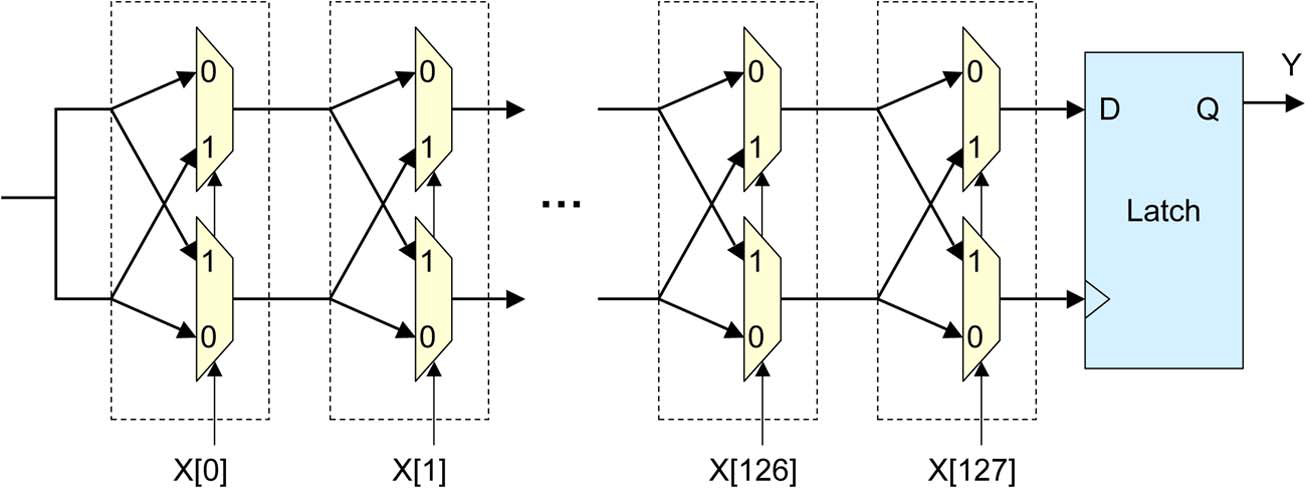
\includegraphics[scale=0.25]{images/arbiterpuf.png}
\caption{Arbiter PUF example circuit}
\label{fig:arbiterpuf}
\end{figure}
As explained in ~\cite{gassend2002silicon} it is possible to implement manufacturing gate delay drawing out a race condition in a symmetric circuits.  Arbiter PUF, in ~\ref{fig:arbiterpuf}, exploited this phenomenon. It is presented by \textit{Lim et al} in ~\cite{lim2005extracting}.\\
Figure \ref{fig:arbiterpuf} shows a path composed by multiple pairs of multiplexers, called switch blocks, which can become straight or switched depending on the selection bit. 
Selection signal comes from the challenge: the path of the signal will vary depending of these values, and despite identical layout, due to manufacturing variability into gates causes the delay variate for each different IC. 
At the end of path, a latch component , called \textit{arbiter} will receive the signal and the input 'D' signal with a certain order and time. 
As explained, the response value depends on the challenge bits: in particular, figure ~\ref{fig:arbiterpuf} shows a challenge of 127 bit that have 1 response bit. This layout can change, for example, a parallel structure with 128 response bit can be build duplicating 128 times the design\\
It must be specified that if the delays are close enough, the latch's set-up time is not enough giving back a non stable output. This phenomenon is called \textit{metastability} and generates noise in the PUF response ~\cite{maes2010physically} . The design is symmetric and does not contain any secret information: even if an adversarial manufacturer owns the design he cannot obtain the same CRPs due to manufacturing variation of each IC. 
Furthermore, the high costs required to evaluate gate delays make the individual delay extraction expensive for invasive attackers. 
Environmental changes effect on Arbiter \puf{} is analyzed in ~\cite{delvaux2013fault}. 
in which is empathized a main drawback in this logic: each delay is independent from other and all the delays are added linearly to each other making possible to create a linear system to model gate delays and generates few CRPs  ~\cite{lim2005extracting}.  
A possible solution consists in the introduction of other \emph{non-linear} effects in order to give a certain error to modelling attacks, i.e. \emph{XOR Arbiter PUFs} or \emph{feedforward Arbiter PUFs}  ~\cite{majzoobi2008lightweight}, ~\cite{suh2007physical}, which anyway are vulnerable against strong machine learning and side-channel attacks as explained in ~\cite{ruhrmair2013power} and ~\cite{mahmoud2013combined}.\\
An Arbiter \puf{} implementation is developed in ~\cite{gassend2004identification} using 23 FPGAs achieving $\mu_{inter} \approx 23\%$ and $\mu_{intra} \approx 99\%$. It is interesting to notice the high reliability and low uniqueness obtained specifying that edge-triggered flip-flops are not fair as arbiter while flip-flops D are a more reasonable choice.
\begin{figure}
\centering
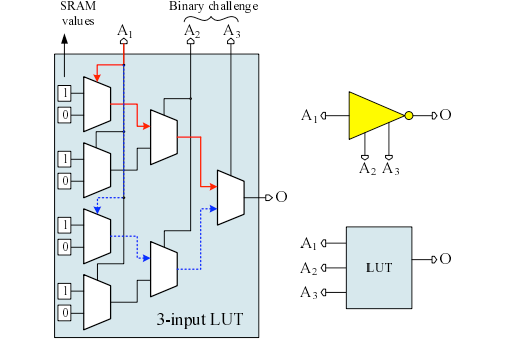
\includegraphics[scale=0.40]{images/pdl1.png}
\caption{Programmable Delay Lines Example}
\label{fig:pdl1}
\end{figure}
\subparagraph{Programmable Delay Lines} \label{par:programmabledelay}
As described before, in order to obtain a response from an IC suitable for PUF use, the signal routing problem have to be controlled. \\
Thus, in \cite{majzoobi2010fpga} \emph{programmable delay logic} are presented. PDL can be implemented into LUT internal structure. Moreover, PDLs perform fine tuning to cancel out delay skews caused by asymmetries in routing and systematic variations, and them can be used for an efficient Arbiter-PUF implementation.
\begin{figure}
\centering
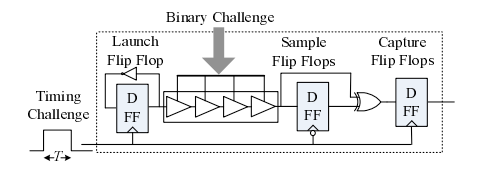
\includegraphics[scale=0.50]{images/delaycharacterizationcircuit.png}
\caption{Delay Characterization Circuit}
\label{fig:pdl2}
\end{figure}
Figure \ref{fig:pdl1} shows LUT configured with $A_{1}, A_{2}$, $A_{3}$ as input. LUT output is $A_{1}$ inverted value where $A_{2}, A_{3}$ are use to determine the path. In figure \ref{fig:pdl1} two paths are shown: blue path provides ($A_{2}A_{3}='00'$) and is longer than the red path with ($A_{2}A_{3}='01'$). Thus, blue path causes a larger propagation delay than red one. 
\begin{figure}
\centering
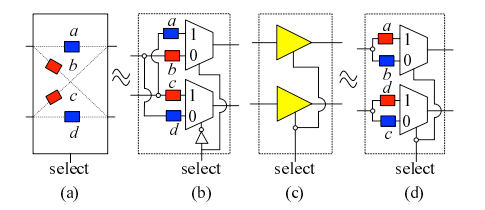
\includegraphics[scale=0.50]{images/pdl2.png}
\caption{Path Swapping Switch with their delay abstraction (a)(b), PDL based switch and its delay abstraction (c)(d)}
\label{fig:pdl3}
\end{figure}
In order to evaluate LUT propagation delay on different inputs, a delay characterization circuit is considered, as shown in figure \ref{fig:pdl2}. This circuit is composed of: a \emph{launch} Flip-Flop, a  \emph{sample} Flip-Flop, a \emph{capture} Flip Flop, a \emph{XOR gate} and a \emph{Circuit Under Test} (CUT).

At the rising edge of the clock a signal is sent through the CUT by the launch flip-flop. At the falling edge of the clock, the output of the CUT is sampled by the sample flip-flop.
If the signal arrives at the sample flip-flop before that sampling takes place, the correct value is sampled. Later, the XOR compares the sampled value with steady state output of the CUT and produces a zero if they are the same. Otherwise, the XOR output rises to ‘1’, indicating a \emph{timing violation}. If the signal arrives almost simultaneously with when sampling occurs, the sample flip-flop enters into a metastable condition and produces a non-deterministic output. By sweeping the clock frequency and monitoring the rate at which timing errors happen, the CUT delay can be measured with a very high accuracy. Resuming, this circuitry can evaluate LUT delay with low-overhead in order to tune and calibrate the delay bias caused by asymmetries in signal routing. Thus structure can mitigate arbiter routing problems. Moreover majority voting and redundancy are introduced to mitigate arbiter metastability problem. 
\begin{figure}
\centering
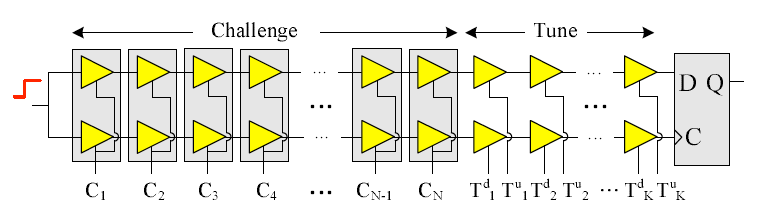
\includegraphics[scale=0.50]{images/improvedarbiter.png}
\caption{Arbiter-based PUF proposed by Manjzoobi et al}
\label{fig:improvedarbiter}
\end{figure}
The Arbiter-PUF structure previously presented uses patch swapping switches, shown in \ref{fig:pdl3} (a)(b). An alternative arbiter-PUF scheme requires perfect layout symmetry, hence, non-swapping switch blocks are introduced \ref{fig:pdl3} (c)(d). 
Basing on these assumptions, an arbiter PUF structure which relies on new switch structure and the tuning blocks is shown in Figure \ref{fig:improvedarbiter}: this structure is composed of N non-swapping switches and K PDLs. 
PDL blocks can be used to distinguish challenges that cause a large delay difference under each different temperature or voltage marking them as robust challenges. But responses of robust challenges can have lower entropy. 
\paragraph{Ring Oscillator PUF} \label{par:ropuf}
Ring Oscillator (RO) ~\cite{suh2007physical} is a delay-based \puf{}, shown in \ref{fig:ringoscillator}. RO design consists of odd inverting gates which permit the maintenance of a continuous oscillation. Signal frequency is related to each inverting stages, which are the cause of delay too. The RO PUF can be synthesized onto Field Programmable Gate Array (FPGA) or an Application-Specific Integrated Circuit (ASIC). 
\begin{figure}
\centering
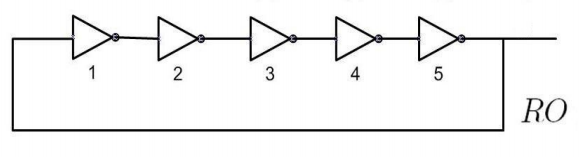
\includegraphics[scale=0.40]{images/ringoscillator.png}
\caption{An example of Ring Oscillator composed of 5 stages}
\label{fig:ringoscillator}
\end{figure}
Ring oscillator behaviour is characterized by different gate delays that involves different frequencies between the oscillators. The frequency of a pair of oscillators are measured and compared: this comparison for each pair generates \puf{} response bits. Given N oscillators, the overall possible pairings are $\frac{N(N-1)}{2}$. A paring strategy may be the following: given N ring oscillators, not all the obtained bits by pairing  are independent. So the entropy\footnote{The term \emph{entropy} indicates the number of independent bits that can be generated from a circuit.} is less than $\frac{N(N-1)}{2}$. For maximizing entropy $\frac{N}{2}$ couples are considered, yielding to a limit upper bound of O(N) challenges.
\begin{figure}
\centering
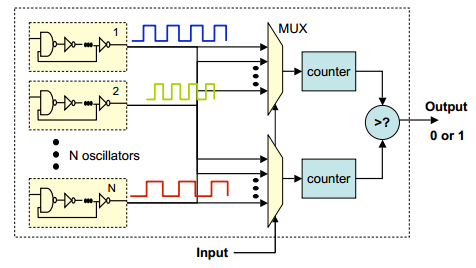
\includegraphics[scale=0.60]{images/ringoscillatorpuf.png}
\caption{Ring Oscillator PUF}
\label{fig:ringoscillatorpuf}
\end{figure}
Ring Oscillator belongs to weak \puf{} category: once the PUF is fabricated, the ring oscillator's frequency is set generating an output string which remains constant. Moreover, RO \puf{} are vulnerable to environment variation and possible workaround to this drawback have to be considered: ring oscillators frequencies far apart are paired each other, avoiding the coupling of neighbouring frequencies.
RO \puf{} is composed by oscillators with close frequencies have bigger error probability than oscillators characterized by distant frequencies.
In ~\cite{yu2010recombination} is described a possible Ring Oscillator PUF architecture. In this architecture, shown in \ref{fig:ringoscillatorsumpuf}, several ring oscillator are divided in k pairs, where each pair have a certain frequency difference $\delta f_{i}$. All the $\delta f_{i}$ can be summed and the challenge bits determine the sign of the $\delta f_{i}$ into the linear combination. The scheme final block compares results of the sum with zero and produces response bits. Using this structure, the number of possible Challenge-Response Pairs increases o $2^{k}$. In ~\cite{maiti2010large},~\cite{maiti2011improved},~\cite{komurcu2013ring},~\cite{feitenanalysis}, RO (Ring Oscillator) \puf{s} have valid good $\mu_{intra}$ while the reliability do not. 
Ring Oscillator \puf{s} relies on cryptographic hardware/software approaches useful to protect security of response bit. There are several malicious approaches that could threaten the RO \puf{} performances: the most common type of attack does not try to steal the key, but to invalidate the response generation. 
\begin{figure}
\centering
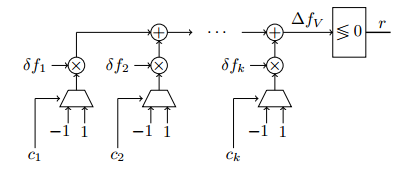
\includegraphics[scale=0.65]{images/ringoscillatorsumpuf.png}
\caption{Ring Oscillator Sum PUF}
\label{fig:ringoscillatorsumpuf}
\end{figure}
In ~\cite{markettos2009frequency} is shown a technique in which sinusoidal signal is driven on the ground plane of a RO in order to lock the output signal: this kind of approach can be also used to invalidate a TRNG behaviour. \\
In addiction, ~\cite{merli2011semi} shows a method in which due to electromagnetic radiation, RO PUF output bits are stolen: a parallelized execution of oscillators can be used to face this attack, in this way, an attacker cannot easily understand which bits snoop.
\paragraph{Anderson PUF} \label{par:andersonpuf}
\begin{figure}
\centering
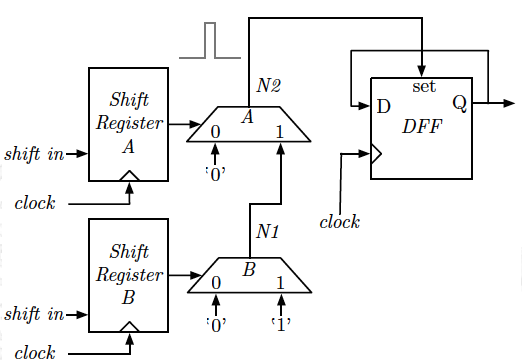
\includegraphics[scale=0.40]{images/andersonpuf.png}
\caption{Anderson Cell}
\label{fig:andersoncell}
\end{figure}
Anderson \puf{} is presented in ~\cite{anderson2010puf}: it is based on logic gates available into FPGAs, but it needs a specific implementation on each FPGA family. Anderson PUF is composed of Anderson PUF cells, which consist of two shift-registers A and B , two 2:1 multiplexers, namely mux-A, mux-B, and one flip-flop D. 
Figure \ref{fig:andersoncell} shows Anderson PUF cell scheme: each cell produces a logic output of '0' or '1', which depends on manufactoring difference between ICs. The mixture of several cells achieves a valid \puf{}  behaviour. Lets now describe how Anderson PUF works: referring to  \ref{fig:andersoncell}, the two shift register, called A and B into the figure, are driven by a clock signal and initialized by means of a signal in opposite phase, i.e. $0x5555$ and $0xAAAA$. 

The two multiplexer are characterized by selection signals respectively driven by the Shift Register B and A. The multiplexer with selection signal driven by B's output have  \emph{logic0} and \emph{logic1} respectively as in 0 and 1 input, while the other one receives the first multiplexer output, $N1$ as input for port '1' and a \emph{logic0} value into '0' input port. The second multiplexer output is defined as $N2$. 

Therefore, the flip-flop D has as input a feedback for D port, N2 for set port and a clock signal. Flip-flop D holds the value which depends on signal propagation and delay. Shift registers A and B outputs are opposite: so, when A outputs is \emph{logic1}, B outputs is \emph{logic0}. The shift registers A and B ara characterized by the same design but a different signal propagation delay, and, this phenomena generates \puf{} unpredictable response. This design requires some additional consideration: 
\begin{itemize}
\item When the delay between A and mux-A is shorter than betwenne B and mux-B, A switches from \emph{logic0} to \emph{logic1}, so mux-A selects the input \emph{logic1} but N1 has not changed its value due to B which does not switch from \emph{logic1} to \emph{logic0} yet.
Therefore, the mux-A output, N2, is determined by the value of N1 which is '1' until shift register transits to '0' as detailed before. During this interval, a \emph{glitch} will appear on N2. 
\item When the delay between couple A is greater than couple B, B output switches from \emph{logic0} to \emph{logic1} while selection value for mux-A does not change. Since N2 value depends on mux-B output, that is N1, a glitch will appear on N2 until the mux-A and A couple switches from \emph{logic1} to \emph{logic0}. 
\end{itemize} 
The differences between delays determine the glitch shape: Anderson explains that the glitch should have a certain duration. If it is too short, the routing network output becomes predictable and generates the same outputs for several FPGAs.
Conversely, the glitch must be greater than the flip flop output set-up. In order to achieve a working Anderson PUF implementation, a \emph{glitch tuning} is required. Without this operation Anderson cells output may be not random and the design can not be targeted as \puf{}.  
Anderson \puf{} is a collection of Anderson cells which work together to generate an unique response that can be used as IC signature.  \\
Anderson PUF is considered as \textbf{FPGA-dependent.}, because depending on the FPGA family used, the cell combination design changes: different implementations have been presented in literature.  \\
In ~\cite{anderson2010puf} Anderson designs its PUF on \emph{ Xilinx Virtex-5 65 nm} shown in figure \ref{fig:andersoncellvirtex}. Anderson PUF cell can theoretically be synthesized on a single slice \footnote{The FPGA perfom logic function by mean logic resource replicated into CLBs. Each CLB can contain slices, a logical elements which contains a set number of LUTs, flip-flops and multiplexer. LUT is a collection of logic gates hard-wired on the FPGA. The slices can be of two types: SLICEL, which implements logic and aritmetic funcions and SLICEM, which provides memory function and operation as a shift-register and RAM}, however, adopting glitch tuning is evaluated that a valid glitch on Virtex-5 technology requires a cell design seized two FPGA slices.
\begin{figure}
\centering
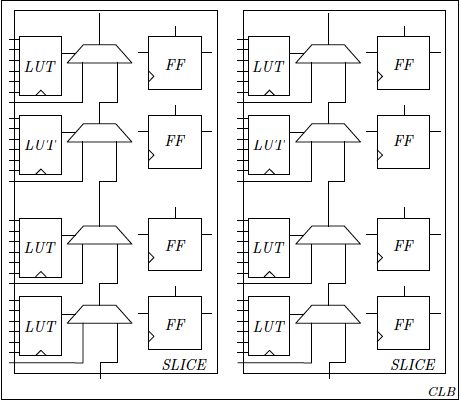
\includegraphics[scale=0.40]{images/andersonpufreal.png}
\caption{Anderson PUF on Virtex-5}
\label{fig:andersoncellvirtex}
\end{figure} 
Anderson measures its PUF, obtaining  $\mu_{inter} = 48.28\%$ and $\mu_{intra} = 3.6\%$ considering 128-bit for response PUF and six FPGAs in six different FPGA regions.  
In ~\cite{barbareschi2015implementing} is shown an Anderson PUF implementation on Xilinx Spartan-3E 90 nm FGPA both in classical form that enhanced. Anderson PUF is characterized by $\mu_{inter} = 47.18\%$ and $\mu_{intra} = 0.15\%$ for the normal version and $\mu_{inter} = 49.37\%$ and $\mu_{intra} = 0.09\%$ for the enhanced one. Enviromental test temperature is $24^{o}$. When enviromental temperature raises to $70^{o}$ \emph{reliabilty} stands around $90.79\%$ in normal form and $98.14\%$ in enhanced form. 
In a successive work evaluates, the impact of the voltage variation on Anderson \puf{}, implemented on Xilinx Spartan-3E family \cite{barbareschi2015supply}.  Experimental results states that the supplied voltage value can dramatically change the quality of \puf{} responses. 
Other Anderson PUF implementation is made on Xilinx Zynq-7000 28 nm FPGAs ~\cite{zhang2013design}, Xilinx Virtex-6 40 nm  ~\cite{huang2013delay}.
The Anderson \puf{} is characterized by the absence of challenge-response pair returning an unique hardware signature. In ~\cite{huang2013delay} is presented and improved version of the Anderson PUF called \emph{Enhanced Anderson \puf{}}, shown in figure \ref{fig:ehnancedanderpuf}. 
This variation adds logic components to Anderson \puf{} design: one shift register and two 2-to-1 multiplexer in order to receive input challenges. 
\begin{figure}
\centering
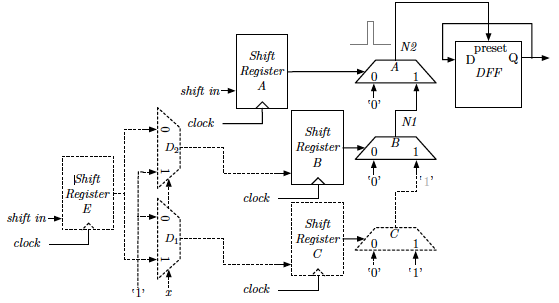
\includegraphics[scale=0.55]{images/ehnancedpuf.png}
\caption{Enhanced Anderson PUF Architecture}
\label{fig:ehnancedanderpuf}
\end{figure} 

\paragraph{ALU PUF}
In \cite{kong2014pufatt} ALU PUF is presented. This type of \puf{} belongs to delay-based category exploiting delay differences between two different Arithmetic Logic Units (ALUs) due to IC manufacturing variations. 
An ALU can be easily find into an processing architecture design and in order to be adapted for \puf{} response generation,  requires minimal component addictions: delay gates and an arbiter. 
The former is composed of programmable delay lines, shown in \ref{par:programmabledelay} with a different delay for each IC due to manufacturing  variation and the latter which choiche a particular bit as response. 
Figure \ref{fig:alupuf} shows an ALU PUF design example with 4-bit operands. An ALU is composed of integrated circuits arithmetic and logic computing. Given two ALUs, each takes the same 4-bit input, first addend is $x_{0},x_{1},x_{2},x_{3}$ and second one is represented by $x_{4},x_{5},x_{6},x_{7}$. Each ALU generates output signals $o=(o_{1}...o_{3})$ and $o'=(o'_{1}..o'_{3}$ : this bits are directed to arbiter generating the response, as shown in figure \ref{fig:alupuf}.
In order to rightly realize the mechanism, both ALUs are characterized by a \emph{Syncronization Logic} which guarantees same computation time for ALU operations. \\
\begin{figure}
\centering
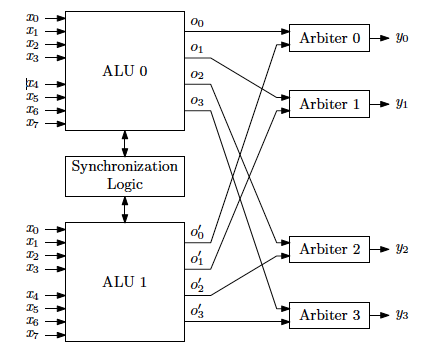
\includegraphics[scale=0.60]{images/alupuf.png}
\caption{ALU PUF example}
\label{fig:alupuf}
\end{figure}
The ALU PUF can be activated running an assembler \emph{add} operation. \\
ALU PUF is experimentally tested on Xilinx Virtex 5 XC5VLK110T FPGA device with a 16-bit model. Two symmetric ALU are implemented together with programmable delay lines (PDLs) realized by mean 64 stages. PDLs occupy considerable area on FPGA. 
In terms of security, ALU PUF shows drawbacks against machine learning attacks: a solution is the addition of XOR-based obsfuscation network. Using XOR obfuscation approach, an adversary cannot directly read the PUF responses. 

Performance evaluation on ALU PUF show $\mu_{inter} = 41.3\%$ with XOR obfuscation and $\mu_{inter} = 18.8\%$ without it . Intra-chip Hamming Distance is around $\mu_{intra} = 18.6\%$. 
Furthermore, ALU PUF response can be suit the role of cryptographic key associated with an error correction mechanism. In \cite{kong2014pufatt} the author uses BCH error correction code. 
\subsubsection{Memory Based PUFs}
In~\cite{su2007isscc} another category of \puf{} is presented: the memory-based \puf{s}. During power-Digital memory storage ,during its power-up, is characterized by a random initial state: it can be demonstrated that this initial state can be considered as a \puf{}. In fact, digital memory implementation is based on bi-stable logic cells, which store one binary digit: once a memory is powered-up in a short time converge to one of its stable state. Each cell tends to stabilize its state to one in particular: memory-based PUFs relies on this behaviour and each memory can generates an unique signature that can be considered as \puf{}. . 
\paragraph{SRAM PUF} \label{par:srampuf}

\begin{figure*}
	\centering
	\begin{subfigure}[t]{.5\textwidth}
		\centering
		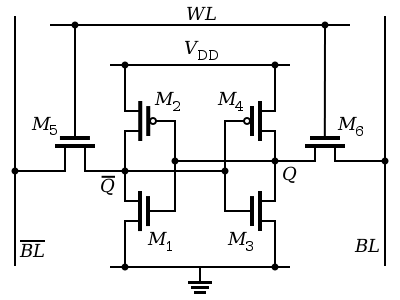
\includegraphics[width=0.8\textwidth]{images/sramcell.png}
		\caption{SRAM six-transistors cell schematic.}
		\label{fig:sramcell}
	\end{subfigure}%
	\begin{subfigure}[t]{.5\textwidth}
		\centering
		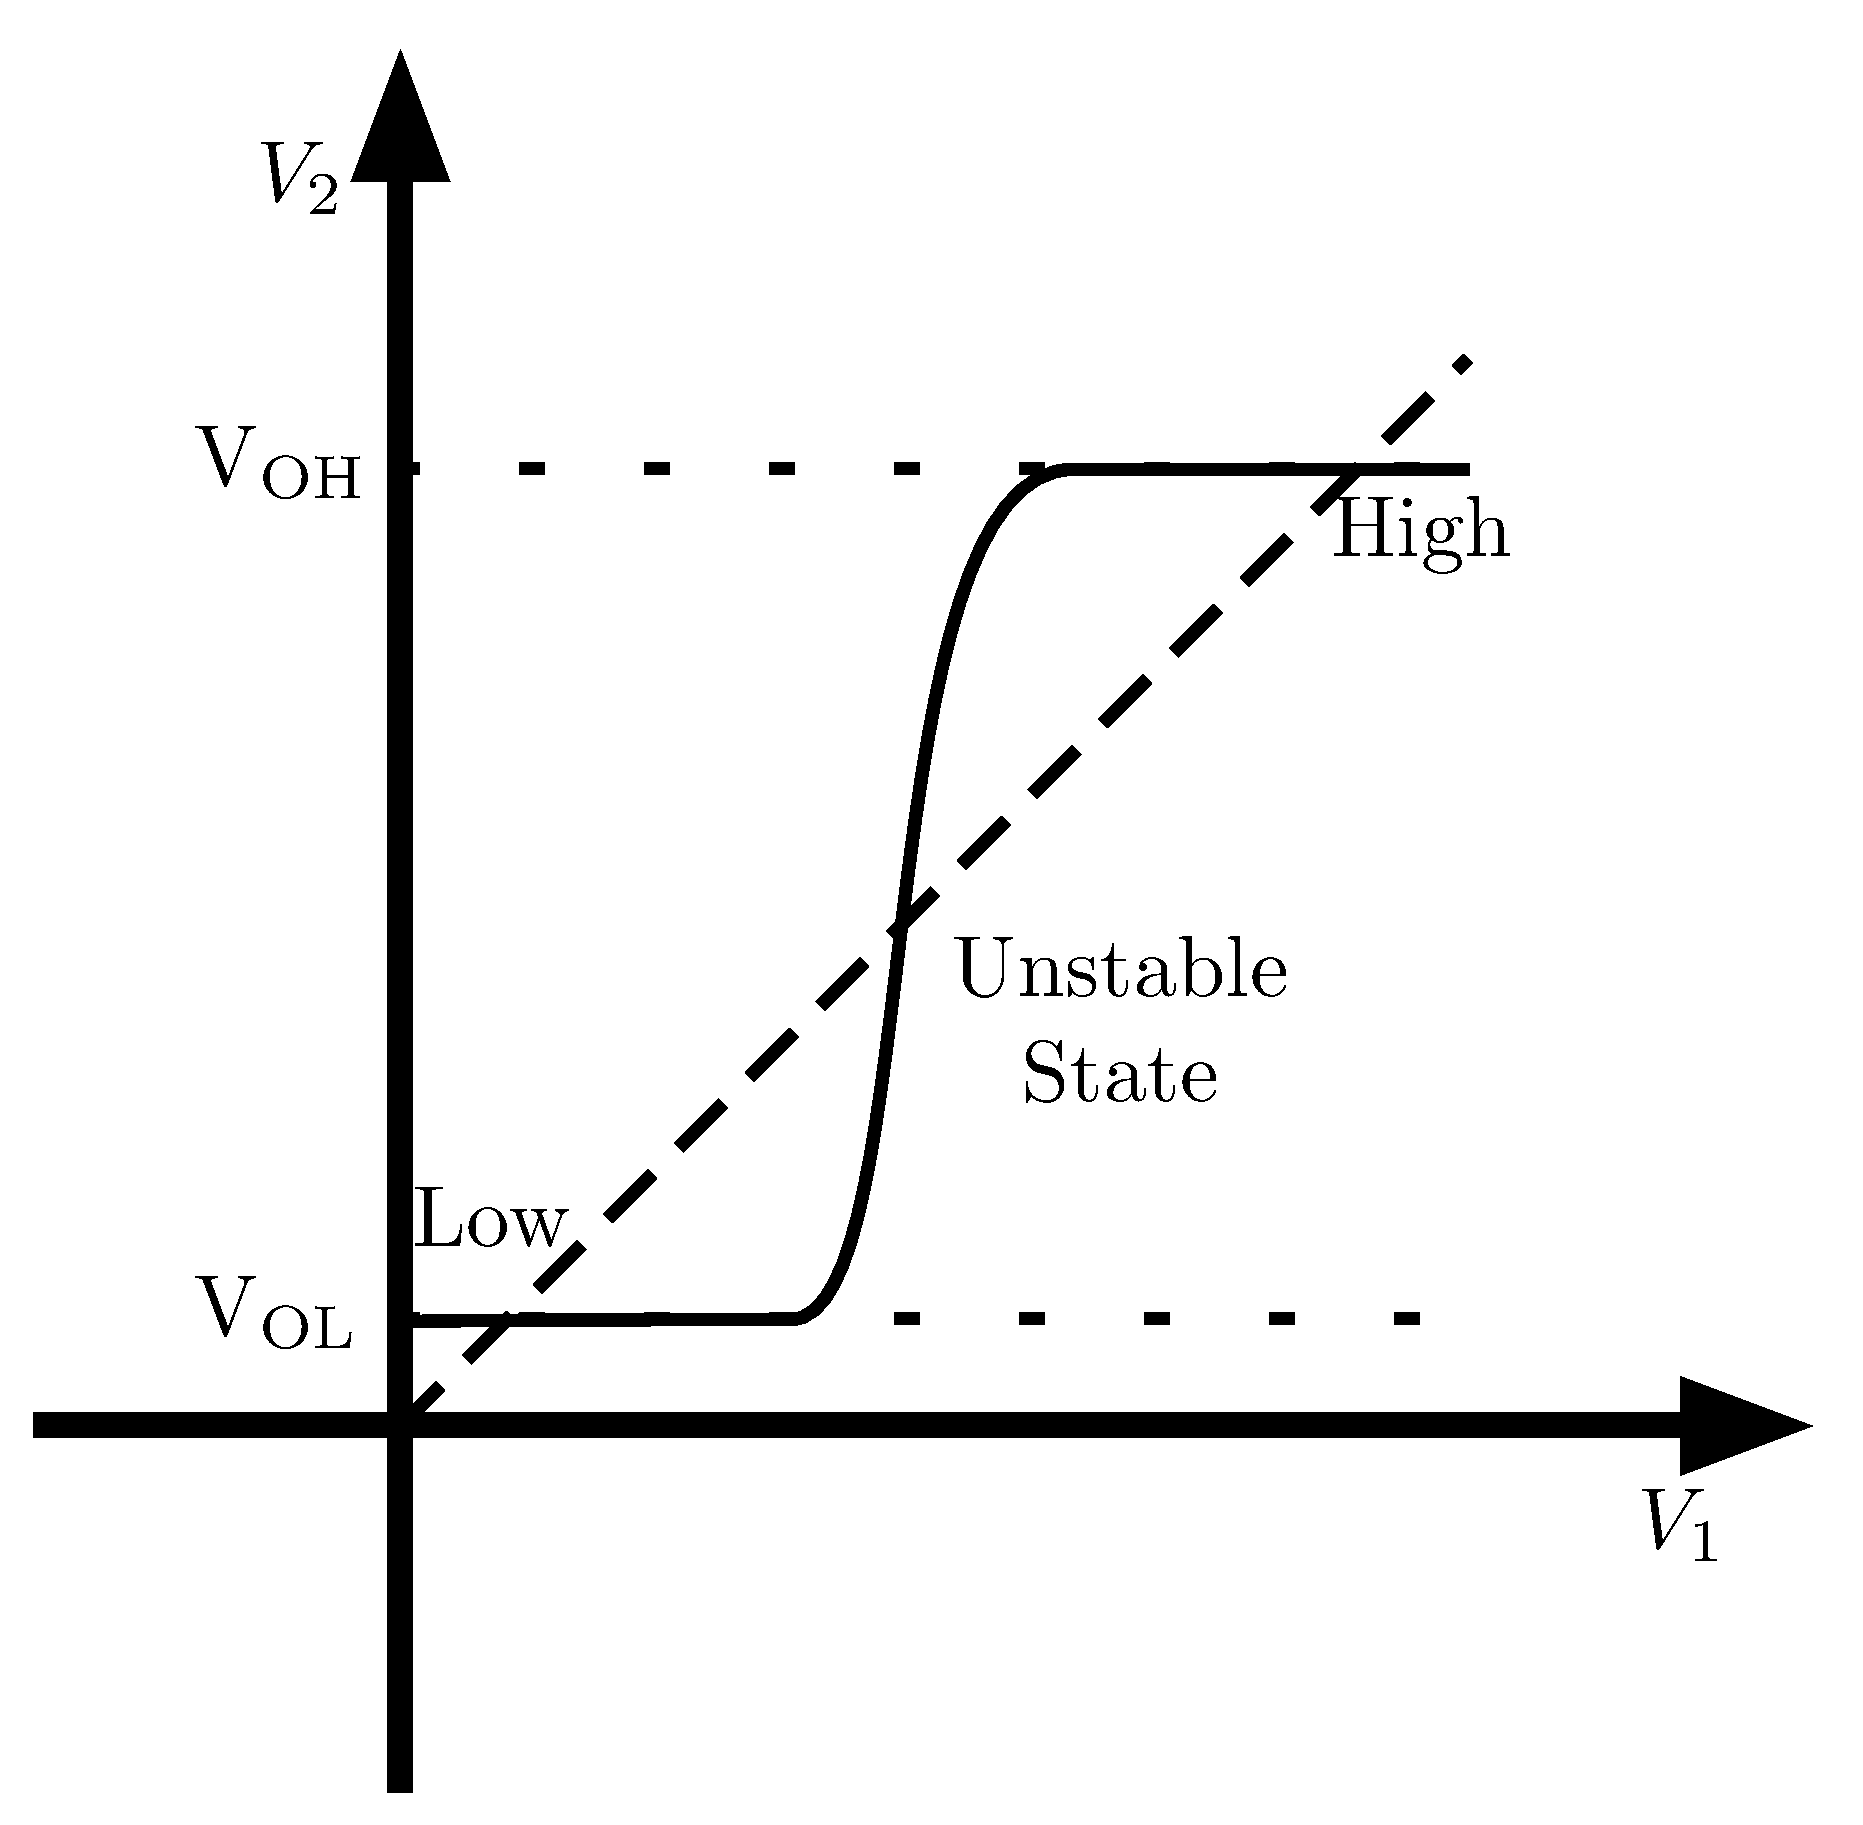
\includegraphics[width=0.8\textwidth]{images/sram_cell_graph.pdf}
		\caption{SRAM input-output voltage graph.}
		\label{fig:sram-graph}
	\end{subfigure}
	\caption{Details of SRAM implementation and input-output characteristic.}
	\label{fig:sram}
\end{figure*}

%% PER ESEMPIO...LA SRAM PUF la dovrei trattare con GRANDE PRECISIONE...prendere info da paper IEJS.
SRAM PUF exploits intrinsic properties of memories. 
SRAM cell is a volatile memory technology commonly used into ICs which loses its content after power-down. The SRAM cell is a symmetric circuit composed of two halves and each one contains an inverter cross-coupled with the other one. Figure \ref{fig:sramcell} shows a schematic for the SRAM six-transistor cell, realized in CMOS technology. SRAM cell is characterized by two stable states whereby it can store `0' or `1', and by one unstable state as illustrated in Figure \ref{fig:sram-graph}. In particular, the SRAM cell keeps the unstable state only when it is powered-up. Due to mismatches between two halves, each cell is forced to a preferred stable state by the inherently positive feedback, realized through the cross-coupling, which amplifies even small voltages variations. As the mismatch between the two halves is imprinted by the manufacturing process, the initial state of each cell cannot be predicted. 

We can classify SRAM cell mismatch configurations by their behaviour at start-up as presented in \cite{cortez2012modeling}: 
\begin{itemize}
\item \textbf{non-skewed cells}, which exhibit a random behaviour due to manufacturing variation effects that are mutually nullified;
\item \textbf{partially-skewed cells}, which are characterized by a mismatch such that they have a preferred state, but it can be influenced by external conditions, such as the voltage;
\item \textbf{fully-skewed cells}, which have a start-up preferred state that, unlike the partially-skewed cells, does not change, even under different external condition variations.
\end{itemize}
Additionally, as stated in \cite{maes2009low}, the amount of cells that very often produce a bit error, i.e. partially-skewed and non-skewed cells, is lower than the number of cells that very rarely produce a bit error, i.e. fully-skewed cells. The SRAM PUF is based on the extraction of a bit sequence stored into a SRAM, which has been powered-up without any writing operations on it. Hence, we can claim that such bit-sequence has attractive for secure purposes.

The idea about the generation of a fingerprint from memory derives from ~\cite{layman2004electronic} and subsequently several experiments are archived to verify its feasibility ~\cite{holcomb2007initial},~\cite{holcomb2009power}. In \ref{fig:sramcell} is shown an example of SRAM cell electronical structure. 

In ~\cite{guajardo2007fpga} Guajardo \emph{et al.} built a SRAM PUF using an FPGA with embedded block RAM memories. Power-up values of a SRAM cells group is considered as PUF response. They fixed the environmental temperature around $20^{o}$ obtaining $\mu_{inter} = 49,97\%$ and $\mu_{intra} = 3357\%$. 
Once of the main issue in the adoption of the SRAM PUF is the need to power-up memory to obtain PUF response. In Xilinx FPGA families this problem is addressable by power gating feature ~\cite{wild2014enabling}. SRAM PUF is revealed strong against side-channel attacks, and modelling attacks if the key is secretly stored. 
Since SRAM PUF is sensitive to noise, in order to produce a stable fingerprint an error correction mechanism is required: in ~\cite{maes2009low} is shown a low-overhead solution.
The Main security drawback of SRAM RAM is level of access: in the event of a change to an environment variable, such as the temperature, the PUF may fail. Otherwise, an attacker who can access to the power channel may modify the stability of the SRAM cells and consequently the \puf{} response. An interesting study is made by Helfmeier \textit{et al.} in  ~\cite{helfmeier2013cloning} where is shown that SRAM power-on state can be observed with \emph{near-infrared imaging} during transient operation. This is a side-channel attack that can steal the PUF response: an attacker reveals the bit sequence and after stores permanently it. 
\paragraph{Butterfly and Flip-Flop PUF} \label{par:butterflypuf}
The feature offered by SRAM \puf{} also affect other memory devices based on the cross-coupled circuits. Supposing to have a circuit useful as a memory such as latch, flip-flops and SRAM cells, figure \ref{fig:butterflypuf} shows an example of a single latch build with two cross-coupled inverters. Due to its nature this circuit transits from an unstable state to a stable state forced by an external inputs. The two coupled gates should be as similar as possible, and any differences are only due to factory random variations. These differences cause a mismatch which leads to an unstable state at the  memory circuits start-up. Then, Flip-Flop and Butterfly PUF have been introduced. 

In ~\cite{maes2008intrinsic} and ~\cite{van2010hardware} is implemented a \emph{a flip-flop PUF} which exploits a specific power-up behaviour. These studies examined that, during power up,  flip-flops on Xilinx FPGA are set with an initial specific random-state which is independent from information stored into the bit-stream. ~\cite{maes2008intrinsic} demonstrates that this behaviour can be considered as PUF useful to realize an unique hardware identifier, evaluating   $\mu_{inter} \approx 50\%$ and $\mu_{intra} \min 5\%$, with the adoption of post-processing computation. 
\begin{figure}
\centering
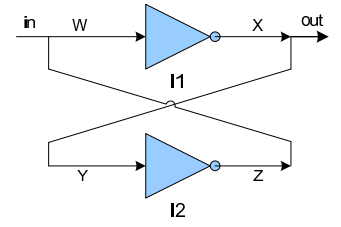
\includegraphics[scale=0.50]{images/butterflypuf.png}
\caption{Cross-Coupled Inverter}
\label{fig:butterflypuf}
\end{figure}
\begin{figure}
\centering
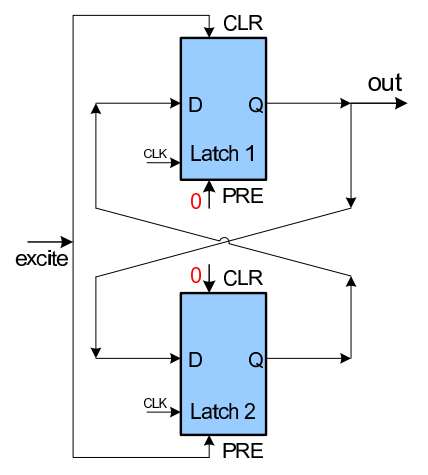
\includegraphics[scale=0.40]{images/ffbutterflypuf.png}
\caption{Butterfly PUF}
\label{fig:butterflypuf}
\end{figure}
At the same way, Butterfly PUF ~\cite{kumar2008butterfly}, is introduced in order to address SRAM PUFs drawbacks. Its design is simile than \emph{latch PUF} ~\cite{su2008digital} design with the difference that Butterfly PUFs can be efficiently implemented on an FPGA while latch \puf{s} do not. In \ref{fig:butterflypuf} is shown the Butterfly PUF logic structure composed by two latch, each with a signals D,Q,CLK,PRE and CLR respectively as input,output, clock, preset and clear signal. In particularly, if the PRE signal value is \emph{logically high} the Q value is set to '1' while if the CLR signal value is \emph{logically high}, Q value is set to '0'. 
For Butterfly \puf{} design, the CLR input of Latch 2 and the PRE input of Latch 1 are always set to low ('0') and  the exepected behavior consider that if CLK signal is high the D value is propagated to Q. 
 
Figure \ref{fig:butterflypuf} shows how \emph{excite} signal that when it is high brings latches having opposite input/output signals and it involves an unstable state into circuit.
When the excite is '0', coupled latch casually assumes one of two possible states with a certain probability. This phenomenon depends on physical differences between gates and wires. 
Butterfly \puf{} can be efficiently implemented on FPGA, in which perfect wiring and gates  symmetry is not reachable.
In ~\cite{kumar2008butterfly} Butterfly PUF on Xilinx Virtex-5 is implemented achieving $\mu_{inter} \approx 45\%$ and $\mu_{intra} \min 6\%$ as performance values.
\subsubsection{Composite PUFs}
Several PUF can be mixed designing a larger one called Composite PUF. Composite \puf{s} has to respect a series of rules in order to obtain a novel \puf{} design with efficient quality parameters. A formal definition \cite{sahoo2014composite} define: 
\begin{quote}
Composite PUF: $\Gamma=\{ \gamma_{i}|\gamma_{i}: C_{i} \rightarrow R_{i}, C_{i},R_{i} \subseteq{0,1}^{+}, i = 1,...,m\}$ is a PUF that is defined by repeatedly applying one or more of the following rules:
\begin{itemize}
\item $\gamma_{i} \triangleleft \gamma_{j} = \gamma_{i}(\gamma_{i}(x))$ where $x \in C_{j}$
\item $\gamma_{i} || \gamma{j} (x,y) = \gamma_{i} (x) . \gamma_{j}(y)$ where $x \in C{i}, y \in C_{j}$ and "." indicates binary string concatenation operation. 
\item $\gamma_{i} \otimes \gamma_{j} (x,y) = \gamma_{i}(x) \otimes \gamma_{j}(y)$ where $x \in C{i}, y \in C_{j}$ and $\otimes$ indicates bit-wise XOR operation. 
\end{itemize}
\end{quote}
An example of \puf{} composition can be founded measuring the space required into different \puf{} combination. However, this solution is not practically feasible and an alternative approach must be adopted.\\
In \cite{sahoo2014composite} is proposed a quality evaluation framework which given quality metrics for a single component grants the possibility to evaluate quality of composite PUF. Howevers, PUF outputs must be independent. The work design a series of composite PUF on Spartan-3 Xilinx FPGA family using as component RO PUF and Arbiter PUF: some are shown in figure \ref{fig:compositepuf}. 
\begin{figure}
\centering
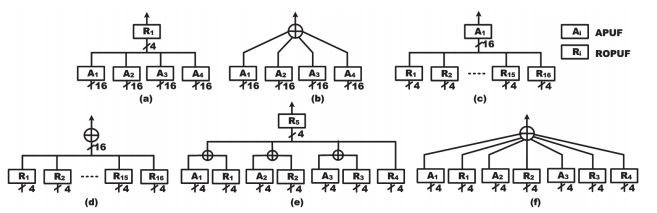
\includegraphics[scale=0.50]{images/compositepuf.png}
\caption{Composite PUF examples }
\label{fig:compositepuf}
\end{figure}
\subsection{Known Attacks Against PUFs and Possible Countermeasures} 
During the previous description of different \puf{s}, several weaknesses are denoted: this section offer a detailed description of the type of attacks on \puf{s}. Depending on the specific type of \puf{}, an attack can be dangerous or not: a \puf{} a immune to all attacks does not exist and, at same time, there is not an attack that could threaten all the types of \puf{s}. 
\subsubsection{Model Based Attack}
% Non dovrei dire cosa sono i model based attacks??
Model based attacks consist in the creation of a model in order to guess response related to specific challenges: this type of attack is mainly directed to strong PUF. Indeed, it is a mistake think that strong PUF with a large number of CPRs can easily avoid attacks. Adopting Machine Learning (ML) approaches, specially algorithms can infer PUF response requiring only few number of CPRs.
An attacker can observe a succession of CRPs acquiring a lot of CRPs: this is a realistic situation where a strong PUF is used. In  ~\cite{ruhrmair2010modeling} several experiments are made showing that with machine learning approach is possible to reveal Arbiter PUF and RO PUF responses with an accuracy near to 99\%. Instead, these attacks do not affect weak \puf{s} because them are not characterized by a large number of useful CRP useful to create a malicious model. 
\paragraph{A Countermeasure against Model based Attacks} \label{par:countermeasuremodeling}
All the malicious attacks are characterized by certain costs:  depending on the situation trying an attack can be a reasonable idea or don't. 

Model-based attacks do not require great costs and it are a valid choice to attack strong PUFs.
In ~\cite{gassend2002controlled} strong \puf{s} drawback against model-based attack is solved combining PUF response with an hash function: the result of this work is the \emph{Contolled PUF} \ref{fig:controlledpuf}. A random hash function is placed before PUF, this countermeasure does not allow a malicious attacker to analyse CPRs. 
\begin{figure}
\centering
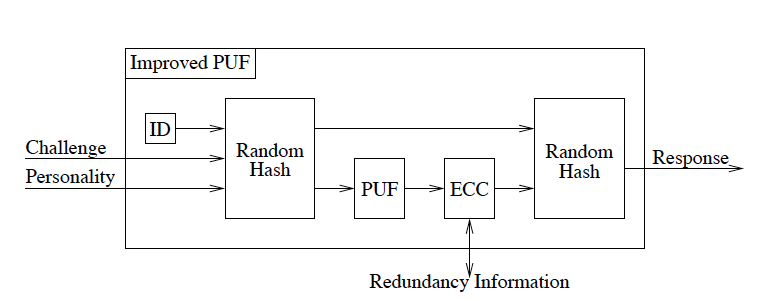
\includegraphics[scale=0.40]{images/controlledpuf.png}
\caption{Controlled PUF generic scheme}
\label{fig:controlledpuf}
\end{figure}
CPR are not used directly: a random function $h$ is used, hence considering $x$ ,$f(x)$ and $h$ respectively as the challenge, the response and the hash functions we have:
\begin{equation}
g(x) = h(x,f(x))
\end{equation}
where $g(x)$ represents the improved PUF response. \\
Hash function application allows to obtain a different response from the original one, and the one-way property of the hash function produces a challenge-response pair which is hard to analyse, even with a large number of couples. A PUF response combination can improve reliability : an attacker cannot see real challenges and additionally, error correction code technique can be considered to transform a noisy PUF response in a more stable value, as shown in figure \ref{fig:controlledpuf}. 
It is important to notice that controlled PUF can be useful to generate is multiple personalities: as we can see in figure \ref{fig:controlledpuf} there is a user parameter called "Personality". Personality parameter can be used to distinguish \puf{} responses with same challenge in different applications: the owner effectively has many different PUFs at his disposal and third parties cannot determine if they interacted with the same device on which a PUF is built. 

Furthermore, in \cite{gassend2002controlled} Gassend \emph{et al} is proposed a method based on controller PUF useful to prevent man-in-the-middle attacks for chip attestation which.
\subsubsection{Side Channel Attack} \label{par:sca}
% Dovrei spendere un paio di parole sui Side Channel Attacks
Side channel attacks (SCA) are a specific attack based on information gained from physical implementation of a security system, i.e a crypto-system in which theoretical strength of implemented cryptographic algorithms is circumvented. For example, timing information, power consumption, electromagnetic leaks or even sound can provide an extra source of information, which can be exploited to break the system. 

Therefore, even the PUF design presents vulnerabilities against side channel attacks. Countermeasures focus to eliminate or reduce the release of side information, as power consumption of timing information or breaking the connection between physical effects and the secret data that security module handles.  However, even if the PUF is protected from SCA, additional post-processing operations do no,  i.e. fuzzy extractor. 
Literature presents some evaluation of side channel attacks on ICs and PUFs:
Power consumption in CMOS technology is caused by state changes hat is the transition of a bit value into IC from 1 to 0 or vice versa. Power analysis attacks exploits this feature: in \cite{ors2003power} this attack is conducted on Xilinx Virtex FPGA family devices.
In ~\cite{karakoyunlu2010differential} is shown SCA which exploited side channel information from a post-processing algorithm. Other work into literature, show how RO PUF response can be recognized using electromagnetic emission relevation. ~\cite{merli2011semi} ~\cite{merli2013localized}.   
At the same time, side channel attacks, which belongs to the category of physical attacks, even though the possibility to affect a wide range of ICs, requires high costs for realization, which reveals a very difficult bond for their implementation.  

\subsection{PUF in Commercial Devices}
Commercial development of PUF is emerging in recent years with security companies that are evaluating inserting them into IC in order to raise device security. \\
\emph{Intrisic-ID} \footnote{https://www.intrinsic-id.com/} was founded in 2008 as a spin-out of Royal Philips Electronics. They patented a PUF technology deployed in Philips production environments applying it in several technology fields as SmartCards, automotive, set-top box, Pay TV applications, networking and communications, mobile, as well as government and military applications.
In 2013 NXP announces a partnership agreement with Intrisic-ID in order to deploy Hardware Intrinsic Security (HIS) adopting \puf{s} into their next  SmartMX SmartCard generation  \footnote{http://www.nxp.com/news/press-releases/2013/02/nxp-strengthens-smartmx2-security-chips-with-puf-anti-cloning-technology.html} available for commercial use within 2014. Furthermore, NXP announces that for the Chinese Market their components will be built into Samsung Galaxy S6 \footnote{http://www.nasdaq.com/press-release/nxp-secure-element-adopted-by-samsung-galaxy-s6-in-worlds-largest-smartphone-market-20150507-00194ixzz3dyQG5aui}.

Altera puts PUF inside their Stratix-10 family FPGA as well as Microsemi\footnote{http://www.microsemi.com/} presents their FPGA families for IoT devices with a built-in PUF. 
PUFFIN project \footnote{http://puffin.eu.org/} intends to study and show the existence of SRAM PUFs and other types of PUFs in standard PCs, laptops, mobile phones and consumer electronics.

Verayo \footnote{http://www.verayo.com/} is a US company which produces secure components for Internet of Things, Trusted Computing and others applications. This company produces low cost authentication solutions using a proprietary PUF technology for digital authentication of products, people and machine. Since 2005 Verayo proposed solutions including unclonable chips, authentication software, consumer engagement, back-end data analysis enabling platforms and key generation. Verayo has ongoing collaborations with US Department of Defense agencies and are based in California. 

\section{Trusted Computing}
%Questa parte subito la appariamo. 
The Trusted Execution Environment (TEE) is a secure area in which some primitives can be executed. Therefore, TEE is an isolated execution environment which provides security functionalities such as isolated execution of trusted applications characterized by integrity and confidentiality guaranteeing more security feature than a Normal Operating Systems operating on a device.
GlobalPlatform \footnote{http://www.globalplatform.org/} and Trusted Computing Group(TCG), non-profit associations, are working to standardize TEE specification: in particular, TCG standardized the Trusted Platform Module (TPM), a security technology which guarantees security features to users. 
Concurrently, industries are working on their own trusted platform as ARM which develops \textbf{TrustZone} for its  A-processors family. 
\paragraph{Trusted Execution Environment}
In \cite{globalplatform2011TEE} GlobalPlatform describes TEE architecture concepts and principles. An Execution Enviroment (EE) is a set of hardware and software components which typically consist of an hardware processing unit, physical volatile memory and non-volatile, peripheral interfaces and connection between processing unit and other hardware resource. An EE can be characterized by security functionalities or not: in former case we speak about Trusted Execution Enviroment (TEE) in the latter of Rich Execution Environment (REE). 
\begin{figure}
\centering
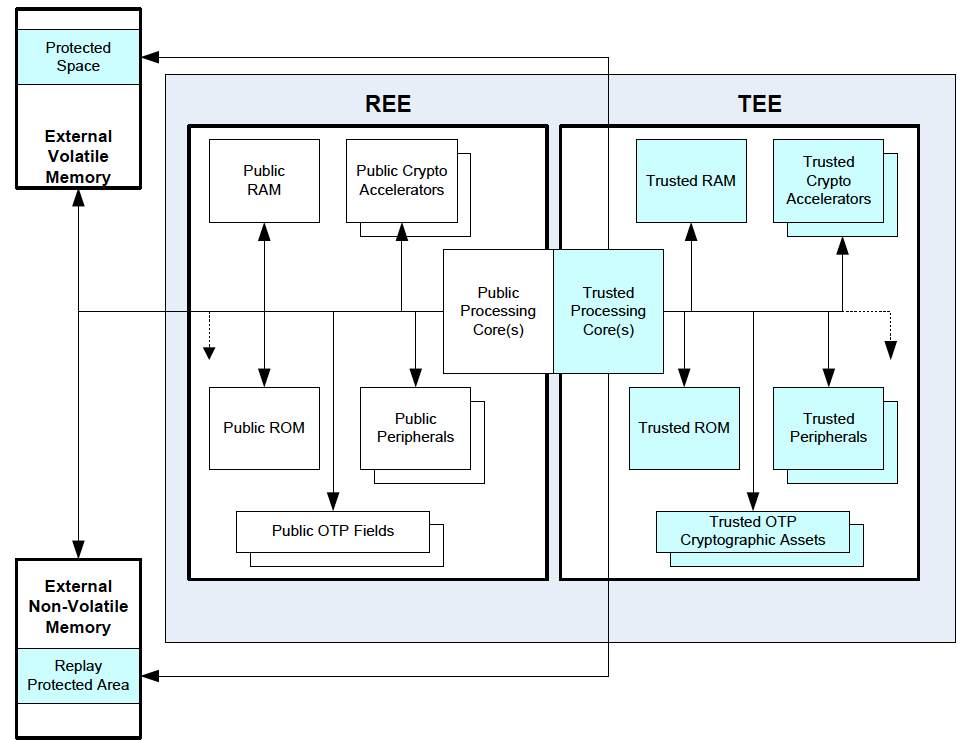
\includegraphics[scale=0.33]{images/teearchitecture.png}
\caption{Hardware Architectural View of REE and TEE}
\label{fig:teearchitecture}
\end{figure}
Typically  client applications run on REE while trusted application on TEE. A Trusted OS is an operating system running on TEE isolating a secure world from a non-secure world. The secure OS manages secure hardware sources, and dispatches the several services which consist in security-sensitive code, while the untrusted word can be considered a mobile operating system such as iOS, Android or Windows 8. \\
If the systems provides one processor, it can only execute one world at time, context switch is required to change execution world. This is done via a special istruction called \emph{Secure Monitor Call (smc)}: when the smc instuction is triggered, the processor switches into a monitor mode that performs the context switch allowing messages exchange between worlds. 
In order to facilitate secure primitive invoking for normal world application, GlobalPlatform consortium develops TEE client API specification \cite{globalplatform2010TEE}.
Software in the REE must not be able to call directly to TEE functions or Trusted Core Framework. The REE can request operation to TEE but it have to go through a protocol verifying the acceptability of the requested operation. Figure \ref{fig:teearchitecture} shows TEE and REE architectural view. REE cannot access to trusted resource, its access is controlled. Trusted resource should be physical isolated from untrusted ones. Figure  \ref{fig:teearchitecture} represents a logical scheme to present separation of secure world from non-secure. 
\begin{figure}
\centering
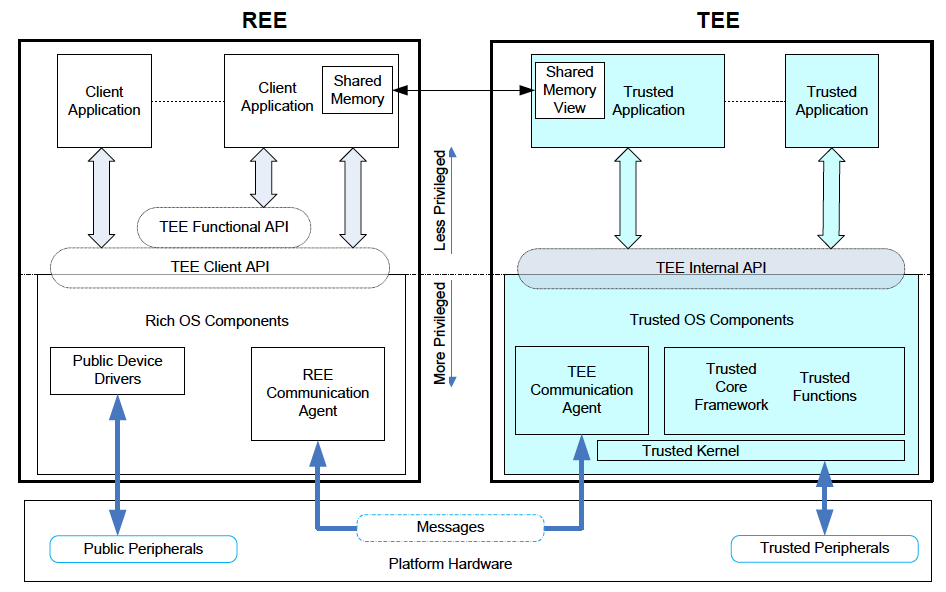
\includegraphics[scale=0.35]{images/teesoftware.png}
\caption{TEE System Architecture}
\label{fig:teesoftware}
\end{figure}
Therefore, TEE offers several APIs to REE allowing it to exploit TEE functionalities. \\
\begin{figure}
\centering
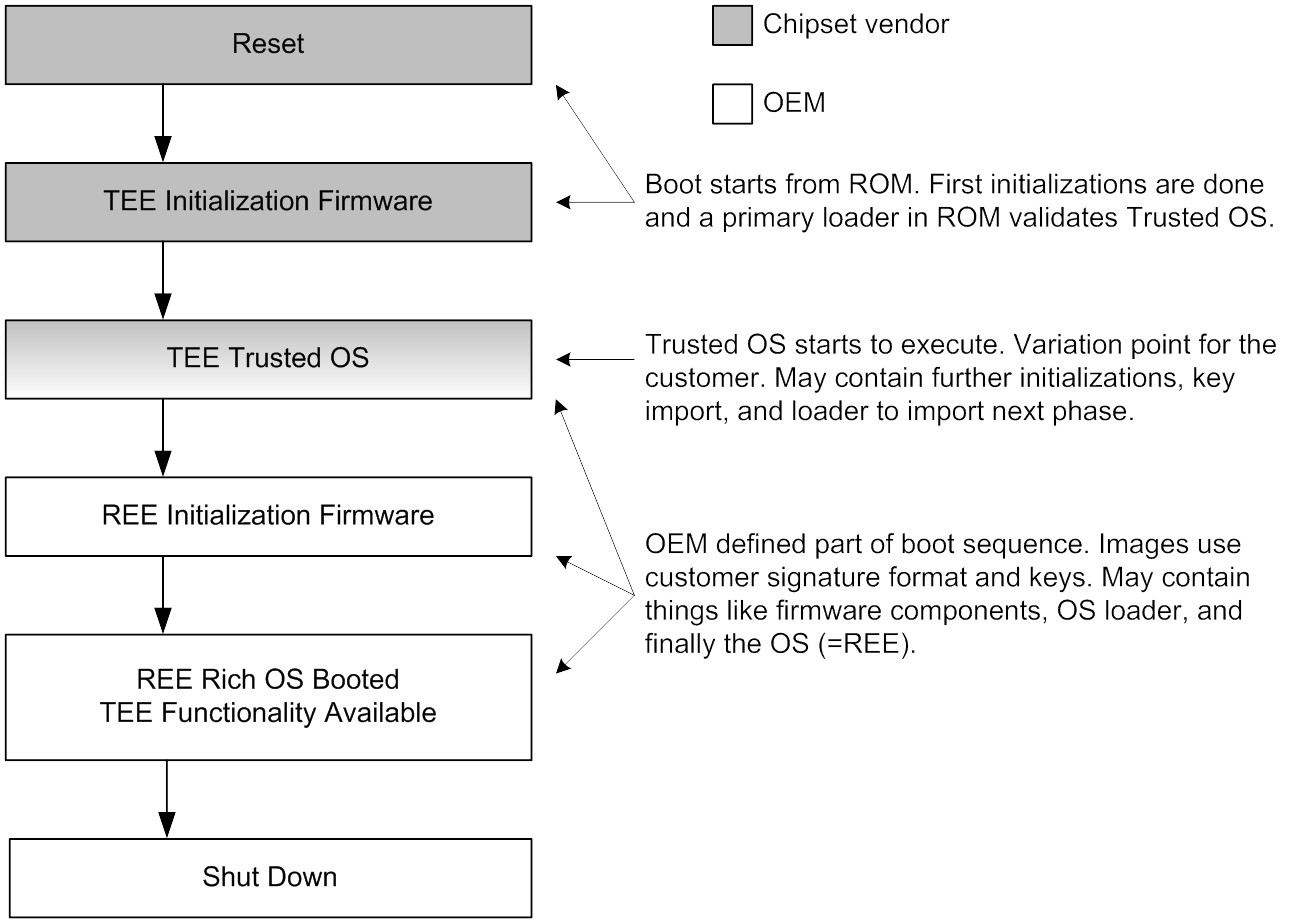
\includegraphics[scale=0.25]{images/teeboot.png}
\caption{Simplified TEE Boot Sequence}
\label{fig:teeboot}
\end{figure}
The relationship between the major software systems components is outlined in the figure \ref{fig:teesoftware}. 
During \emph{Boot Time} the overall hardware powered-up and EE operating system is initialized and loaded into hardware system. For a TEE is required a trusted boot code. Trusted boot includes firmware code that takes control of execution after resetting. A simplified boot sequence flow diagram is shown in figure \ref{fig:teeboot}. 
In order to maintain the chain of trust, TEE can be instantiated either during secure boot sequence or later by software component already instantiated and characterized by  trust level similar to TEE. 

\subsection{Trusted Platform Module}
Trusted Platform Module (TPM) is a chip designed to guarantee security feature on an user platform. The technology was in the early days around 2003 known by the name TCPA (Trusted Computing Platform Alliance), or by the project (and team) names in Microsoft, “Palladium”, or “Next Generation Secure Computing Base”.  The Trusted Computing Group (TCG) was announced as the successor of TCPA, with the partnership of big players in the PC ecosystem: Intel, IBM, HP, AMD and Microsoft. TPM can today be considered a global effort to bring trusted computing, especially a hardware root of trust,
into the personal computing ecosystem

The first specification of the TPM was in 2001, currently there is a draft version of the TPM 2.0 specification \cite{tcg2014_2.0}. 
TPM can be considered as a stand-alone discrete chips which provides a set of security
functions for the operating system and its applications. The TPM interface is a set of functional APIs for security services carried out in isolation, i.e., inside
a Trusted Computing Base (TCB).
TCG specifies TPM requirements for desktop PC motherboards plug-ins and recently releases a specification of trusted module suitable to embedded device, the Mobile Trusted Module \cite{tcg_mobile_1.0}. For resource-constrained devices, it is considered a software implementation of security functionalities without the adoption of a dedicated hardware component. Furthermore, the MTM specification adds some mobile specific functionalities and declares (mandatory) TPM features optional in order to minimize the footprint of the module.
In addition,  TCG proposes trusted computing specification for several applications, as for automotive \cite{tcg2015automotive} or eHealth  \cite{grossmann2007security}.
In \cite{pearson2003trusted} \emph{a trusted entity} can be defined as: \textit{an entity which always behaves in the expected manner for the intended purpose}. \\
Figure \ref{fig:tpmstructure} shows TPM structure as presented in 1.2 TPM Specification \cite{tcg2011main} where the main components are:
\begin{figure}
\centering
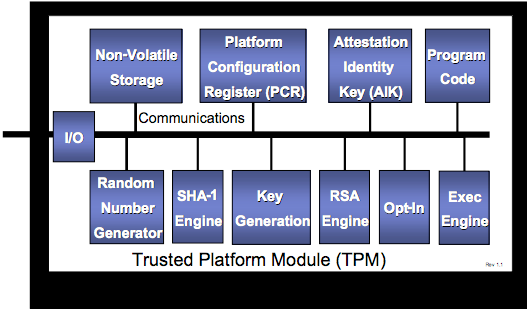
\includegraphics[scale=0.55]{images/tpmv14.png}
\caption{TPM component structure}
\label{fig:tpmstructure}
\end{figure}
\begin{itemize}
\item Input/Output (I/O): This component manages information flow over the communication bus. It routes messages to appropriate component and vice versa, when is necessarily adapting message encoding/decoding them;
\item Non-Volatile Storage: A component which stores asymmetric RSA \cite{jonsson2003public} keys used only inside TPM;
\begin{itemize}
\item Endorsement Key (EK): an TPM unique identifier embedded during manufacturing phase.
\item Storage Root Key (SRK): To reduce the amount of non-volatile memory needed inside the TPM, only one key, namely the SRK, needs to be permanently stored inside the TPM. Other
keys maintained by the TPM can be “wrapped” (encrypted) under the SRK or by another storage key that is already maintained by the TPM. These wrapped keys are maintained outside the TPM by the TSS, which typically stores the keys on hard disk. This allows the TPM to maintain a virtually unlimited. 
\end{itemize}
\item Platform Configuration Registers (PCRs): a trusted memory area in which actual configuration of platform are stored. The information of platform consists in 160-bit hash values. PCRs can be realized by beans of either volatile or non-volatile storage. 
\item Program Code: The firmware for measuring platform devices.
\item Secure Hash Algorithm (SHA-1) \cite{eastlake2011us}: Generates message, that are digest for the PCRs that is the response of an Hash function.
\item True Random Number Generator(TRNG): This components provides, random number for key generations or authentication operations.
\item RSA Key Generation: TCG standardizes the use of RSA algorithm in TPM modules. This component creates signing key (EK) and storage keys (SRK).
\item RSA Engine: This component is used for signing with EK and encryption/decryption of the data with SRK. 
\item Opt-In: This component implements TCG policy requirements for TPM modules shipping and it determines the possibility of using or not a certain module by the customer. 
\item Execution Engine: a component which runs program code.
\item Hashed Message Authentication Codes (HMAC): a component which checks correctness and integrity of a received message for authentication implementing signature mechanism. 
\end{itemize}
\paragraph{TPM implementations in commercial devices}
In spite of this description, TCG does not specify a technology infrastructure to fully utilize this architecture. However, TPM is implemented by several vendors, ATMEL manufactures TPM devices compliant to TCG specification while Infineon provdes both TPM chips and software deliveres as OEM version in new computers. Acer, Wipro, Asus, Elitegroup, Dell, Inc., Gigabyte Technology, IBM, LG, Fujitsu, HP, Lenovo, MSI, Panasonic, Samsung, Supermicro, Sony, Eurocom Corporation, and Toshiba provide TPM integration on their devices and Google includes TPMs in their Chromebook Line-up \footnote{http://chrome.blogspot.se/2011/07/chromebook-security-browsing-more.html}. 
Microsoft has announced that from January 1, 2015 all computers will have to be equipped with a TPM 2.0 module in order to pass Windows 8.1 hardware certification.[24] However, in a December 2014 review of the Windows Certification Program this requirement was changed to optional. However, TPM 2.0 is required for connected standby systems.

The taiwanese manufacturer MSI, lauches its tablet Windpad 110W that is composed of AMD CPU and Infineon Security Platform TPM. Default settings disabling the component but with pre-installed software it is allowed enabling and using it \footnote{http://www.msi.com/product/windpad/WindPad-110W.html\#hero-overview}. 
 
MTM specification does not consider an external dedicated trusted module chip, for this reason, for the field of mobile devices the common approach for building a trusted area on the devices relies on software implementation in secure areas of the memory. For example, TrustKernel's T6 secure operating system simulates TPM functionalities for  mobile devices using the ARM TrustZone technology \footnote{https://www.trustkernel.com/}


\subsubsection{Trusted Module Remote Attestation}
\paragraph*{Integrity measurement}
During the description of the TPM components, has been presented that the role of the PCR for the maintenance of platform integrity measurement: this term as definite by TCG is the \emph{the process of obtaining metrics of platform characteristics that affect the integrity (trustworthiness) of a platform, and putting digests of those metrics in
shielded locations (called PCRs)”}. Hence, PCRs allow to store measurements of the platform state which consists in a cryptographic hashes of all software components loaded during the boot process. The Core Root of Trusted of Measurement (CRTM) , the first code executed by the platform, measure (compute hashes) the code and extend the first PCR register with this measurements and next, another executing code, i.e. the BIOS measure the binary image of the bootloader before transferring execution control to it, storing measured data into another PCR. Therefore, PCRs represented an accumulated measurement of the history of all the code that has executed from the power-up of the platform. CRTM is considered as a \emph{root-of-trust}, a component that must always behave in the expected manner, because its misbehaviour cannot be detected. CRTM together with Root of Trust for Storage (RTS), a computing engine capable of maintaining an accurate summary of values of integrity digests and the sequence of digests , and Root of Trust for Reporting (RTR), a computing engine capable to reliably reporting information held by the RTS, are the root-of-trusted required to build a Trusted Platform. 
\paragraph*{Attestation with Privacy CA}
The roots of trusted described above require certification useful to demonstrate that the platform can be considered trusted. The trusted platform stores keys and other security data object into Protected Location within its own architecture and for this reason it must guarantee its secure nature to build a root-of-trust allowing the building of reliable services for both the user and the provider.
In particular, integrity measurement can be used to ensure platform trustworthiness by logging changes to platform state: it records logged entries in PCR for validation. 
Some certifications are required to establish trust, i.e. for demonstrating that the key creation and protection procedure meets some security criteria. Some keys embedded into TPM's non-volatile memory requires a valid certification to attest their trustworthiness. 
Hence, in \cite{tcg2007specification}, TCG describes how the TPM can provide a remote attestation of the complete platform configuration relying on a Privacy Certificate Authority. 
In particular, with \tpm{}, a device can remotely {\em attest} its trustworthy nature
and prove to a remote-third party verifier that the platform has a specific configuration. 
%
The first attestation method presented by TCG relied on a {\em Privacy Certification Authority}~ \cite{tcg2007specification}, or Privacy CA, a trusted third party in charge of guaranteeing trust among several parties. The platform identity is handled adopting the Attestation Identity Key (AIK) which is created by means of a key certification protocol between user and Privacy CA. 
TCG recommends to store AIK in a persistent internal storage outside TPM where its purpose is providing user privacy when communicating with different sources. T
he AIK adoption is realized to avoid the use of EK with communication with other entities: since the EK is uniquely identifies the TPM, it is a sensitive data that should be shared outside its secure perimeter only when strictly required . An EK theft could lead to attest as trusted a malicious entity that is not. The AIK credential is a certification containing the AIK public key which proves that the corresponding private key is bound to a genuine TPM. This proof
is guaranteed by a signature on the credential created by the Privacy CA. The AIK key pair generation requires several step: (i) the user send a request to Privacy CA together with the endorsement credential, (ii) if the endorsement credentials verification succeeds the Privacy CA creates and signs AIK credentials encrypting them by means on public endorsement key of the platform, in this way the AIK credentials can only be used by platform who required them.
The AIK can be used to sign PCR registers contest and for attesting platform trustworthiness: a third party which is aware of public AIK credentialn can verify the platform identity requesting an integrity report signed the the private part of AIK. 

This approach suffers from two main issues: the Privacy CA must actively participate to each attestation, becoming a bottleneck, and if the Privacy CA establishes a malicious relationship with a third party, the \tpm{} privacy may be compromised. This can happen because each third party entity can obtains identity information about the specific platform when communicates with it: some workaround on the adoption on Applications Identity Keys are proposed in literature, but, any pseudonym used to communicate permits to trace the platform. 

\paragraph*{Direct Anonymous Attestation}
Starting from 1.2 specification \cite{sumrall2003trusted}, TCG proposed an additional attestation mechanism, the {\em Direct Anonymous Attestation} (DAA), introduced by Brickell, Camenish, and Chen~\cite{brickell2004direct} to overcome the drawbacks of the previous attestation mechanism. The attestation approach based on Privacy CA establishing a trusted relation among parties relying a trusted part, conversely, DAA allows to set up a trusted relatioship among parties without the mandatory participation of a trusted one and respecting the user's privacy. 
DAA is based on group signature~\cite{chaum1991group}, enabling users to authenticate their participation in a group of trusted members without disclosing their own identity. Later, several DAA-based schemes were suggested in the literature. 

The DAA scheme involves three players, namely: the Issuer, (TTP), the Device and the Verifier (AS). The DAA protocol requires the Join phase: the Issuer grants credentials allowing
Devices to generate anonymous signatures. Once the Device is able to anonymously certificate its own platform, the Sign phase can take place: messages are signed by the Device and sent to the Verifier using the DAA credentials. During the sign verification, the Device privacy is guaranteed as only the Issuer knows its identity. The Verifier checks if the signature belongs to the DAA group, and consequently, ensures that it came from a trustworthy Device. In order to face the real-word scenario in which TM can be compromised, DAA consider the credential revoking to rogue TM.

The DAA firstly proposed in ~\cite{brickell2004direct} relies on RSA primitives to construct the anonymous group signature. However, in order to increase computing efficiency and reduce the length of the involved group signature, a DAA scheme based on ECC (i.e. ECC-DAA) and bilinear maps is proposed in~\cite{brickell2008new}.
In particular, the research efforts have been focused on balancing the computational load between hosts, an high-end platform, such as a system based on x86/x64 processors, and an embedded resource-constrained \tpm{}.
In order to limit the computation load on the \tpm{}, a few alternative ECC-DAA schemes were proposed~\cite{chen2009daa,brickell2010pairing}.
Indeed, DAA schemes can be also adapted to resource constrained devices as proposed by Ge et al.~\cite{ge2007direct}. 
In the last \tpm{} specification, the 2.0 draft~\cite{tcg2014_2.0}, the TCG includes multiple ECC-DAA schemes.
A comprehensive description of DAA implementation details and its steps which leads to establish an anonymous trusted attestation is presented in [INSERIRE RIFERIMENTO APPENDICE].
 
\subsection{Research Efforts on Trusted Platform into Embedded Systems}
\begin{figure}
\centering
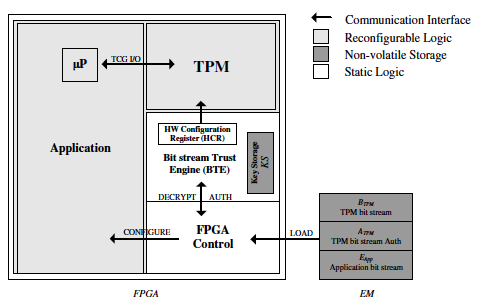
\includegraphics[scale=0.40]{images/eisenbartharchitecture.png}
\caption{FPGA Trusted Architecture proposed by Eisenbarth et al}
\label{fig:eisenbartharchitecture}
\end{figure}
As described above, a trusted component have to be characterized by a CRTM, the first code execute for booting the platform, into PC systems it is usually the BIOS. 
In \cite{eisenbarth2007establishing} Eisenbarth proposed a TPM architecture on FPGA introducing the BitStream Trust Engine (BTE), shown in figure \ref{fig:eisenbartharchitecture} . BTE allows loading, decryption and authetication of bitstream for including configuration bitstream into a chain of trust. 

Furthermore, BTE provides a secure non-volatile key storage (KS) to build a trusted are working together with an Access Control Logic (ACL). ACL relies on BTE credential for protecting bitstream from unauthorized (VERIFICARE IL TERMINE) synthetization. 
If the verification successfully succeeds, the bitstream is loaded into reconfigurable area after a decryption.
 
Eisenbarth's approach requires modification to FPGA architecture to realize BTE, not feasible on FPGAs available on the market.

In \cite{glas2009configuration} is explained how complete TPM integration into a FPGA is not feasible due to volatile nature reconfigurable devices. Then, the realization of FPGA-based TPM needs structural modification into FPGA's design.

\begin{figure}
\centering
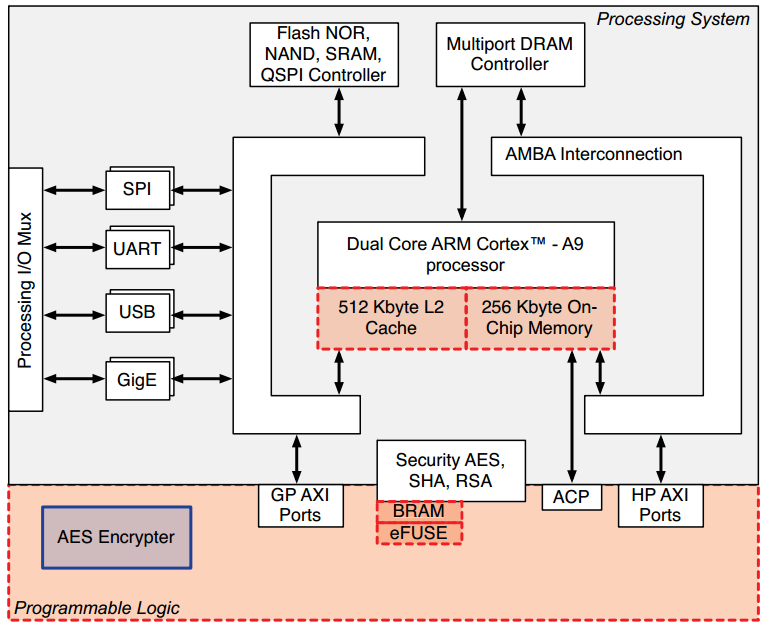
\includegraphics[scale=0.32]{images/zynqarchitecture.png}
\caption{Xilinx Zynq-7000 Architecture}
\label{fig:zynqarchitecture}
\end{figure}
In \cite{barbareschi2014advancing} is realized a chain-of-trust on FPGA technology. As explained before, TPM needs a secure hardware perimeter and FPGA could not satify this requirement without additional components. 
Xilinx Zynq 7000 FPGA/SoC family provides a secure key storage based on Battery RAM (BRAM) and eFUSE and includes an Artix-7 FPGA and processing system dual-core ARM Cortex-A9. 
Figure \ref{fig:zynqarchitecture} shows Zynq internal architecture which natively supports secure system deployment: the orange part indicates the mentioned secure hardware area where keys can be securely stored allowing to build a chain of trust starting from hardware to software.

The secure boot procedure can be considered as root-of-trust: when ARM processor starts, it executes code into ROM: this code is provided by Xilinx and is unmodificable. As explained before, Zynq 7000 provides two secure storage services useful to store master key: BBRAM and eFUSE. During start operations processor verifies whether the key stored in eFUSE/BBRAM matches with key into Boot header. If this check fails, the device transits into a secure lockdown state. 
Conversely, the First Stage Boot Loader (FSBL) is parsed to retrieve boot-code location and actual boot configuration. The storing operation can be encrypted or not, the former case needs decryption operation with AES/SHA modules before loading, the latter do not.
FSBL loads bitstream which configures programmable logic and the user application. All this mechanism guarantees the building of a chain of trust, shown in figure \ref{fig:zynqchainoftrust}. 
\begin{figure}
\centering
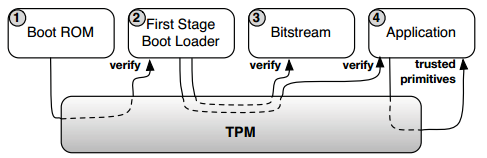
\includegraphics[scale=0.40]{images/zynqchainoftrust.png}
\caption{Xilinx Zynq-7000 Chain of Trust with TPM}
\label{fig:zynqchainoftrust}
\end{figure}

Another approach to build a secure area on reconfigurable hardware is proposted by Glas \emph{et al} in \cite{glas2009configuration. This appoach mantains flexibility advantage of reconfigurablity and at same time respecting Trusted Computing requirements. In particular Glas focuses his work on Xilinx Devices which provide partial bitstream configuration. The main issue is to build a trusted boot system that loads a configuration bitstream containing TPM components. In the proposal, Hardware Configuration Registers (HCRs) are presented, these registers  work together with PCRs presented into TPM basic structure. Proposed design is composed of FPGA architecture with an attached \emph{Trust Block} and a modified JTAG interfacing ($\mu JTAG$).  \\
\begin{figure}
\centering
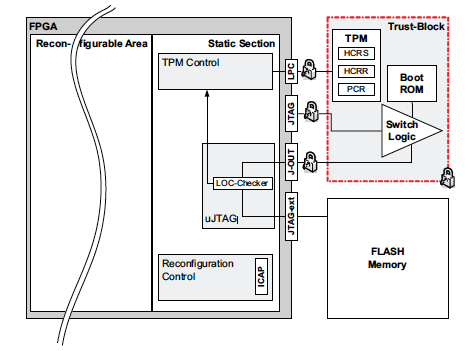
\includegraphics[scale=0.45]{images/glasprototype.png}
\caption{TPM on FPGA with Trust Block}
\label{fig:glasproposal}
\end{figure} 
Trust-Block cointains security relevant parts of the system and it have to be implemented with an external hardware component. Trust-Block interacts with FPGA and its interface must be reliable. Figure \ref{fig:glasproposal} shows TPM architecture: LPC is the Low Pin Count bus interface and connects TPM to FPGA. \\
Into Trust-Block, \emph{secure BootROM} contains the initial bitstream for the device, it is assumed that it cannot be altered after its storing. Moreover, it has been previously validated and certified. Furthemore \emph{integrated switch logic} allows configuration during power-up only from BootROM. 
\\ As shown in figure \ref{fig:glasproposal} there is a Static Section and a Reconfigurable Area upon TPM on FPGA. The former contains the necessary components to build trusted platform that are: TPM Control Block, FPGA-readout functionality and the uJTAG implementation. The proposed JTAG implementation provides the user with an external accessible programming port. it is called JTAG-ext. All data coming from this port are scanned and a targeted reconfigurable area of FPGA is detected. 
\\ System operations follow:
\begin{enumerate}
\item At Power-up the FPGA is configured with configuration bitstream from BootROM (acting as CRTM).
\item HW configuration of both the static and reconfigurable part is read out, stored and hashed into HCRS and HCRR respectively. The same for the software part as specified by TCG. 
\item Using uJTAG port a partial configuration may be made.  All incoming bitstreams are monitored: if an illegal area of FPGA is targeted the TPM is immediately disabled. 
\item When trust authentication is required the TPM sends the requested contents of its secure registers, HCRR, HCRS and appropriate PCRs signed with a secret key. 
\end{enumerate}
In \cite{glas2009configuration} the work shown above is extended with additional and more detailed specifications on the architecture and structure of the components for the static area and the Trust-Block. Microblaze processor plays the role of TPM Control together with a SHA-1 engine and LOC checker module: only Static Section is been implemented. This synthesis occupies $50\%$ of Virtex-II Pro area.\\
Choi shows a PUF-based TPM  chip \cite{choi2012design} (figure \ref{fig:choiproposal}) . This architecture do not use FPGA. The proposed scheme uses PUFs to generate keys used by RSA/AES module. 
\begin{figure}
\centering
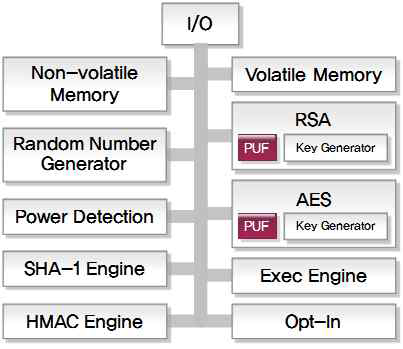
\includegraphics[scale=0.40]{images/choiarchitecture.png}
\caption{Choi's TPM architecture using PUF}
\label{fig:choiproposal}
\end{figure}
So far several TPM implementation are presented, \cite{glas2009configuration} is described an hybrid one that combines previous approaches.

\paragraph{TinyTPM}
\section{An example: Tiny TPM}
Feller et al. proposed a cryptographic model called TinyTPM which enforces trustworthy operation and IP Core protection for embedded systems. TinyTPM can be synthesized on FPGA achieving two main operation: attestation of embedded system state and IP Core protection by providing authenticated and encrypted update procedures for FPGAs. TinyTPM has been designed to require a low quantity of resources well-adapting to the field of low cost FPGA-based embedded system. 
\begin{figure}
\centering
\includegraphics[scale=0.50]{images/tinyTPM.png}
\caption{TinyTPM Architecture}
\label{nome}
\end{figure} 
TinyTPM follows canonical TPM architecture but to save an resources allocated uses cryptographic engines for encryption/decryption as well as for hash and HMAC computation, which are all based on a single block cipher, AES. This choice makes TinyTPM a lightweight module in comparison to a conventional TPM guaranteeing same security efforts (forse un po troppo generico). Into TinyTPM architecture Bitstream Configuration Register replace the Platform Configuration Register playing the same role with the difference that them contains integrity measurements (hashed value) of dynamically loaded bitstreams. An additional BCR is available to record the initial bitstream configuration of the FPGA considering both, static and dynamic logic. \\
This solution provides keys stored into NVM. NVM is used alto to store bitstreams for partial reconfiguration. Key management has been kept deliberately simple and only one key is used for the protection of all IP Cores. Real world applications require individual keys for each IP Core. TinyTPM makes integrity measurements with hash computation, storing calculated values into BCRs. Attestation is made using hashed value of IPCores stored into BCRs issuing these value to a challenger that want to verify system trust. \\
\begin{figure}
\centering
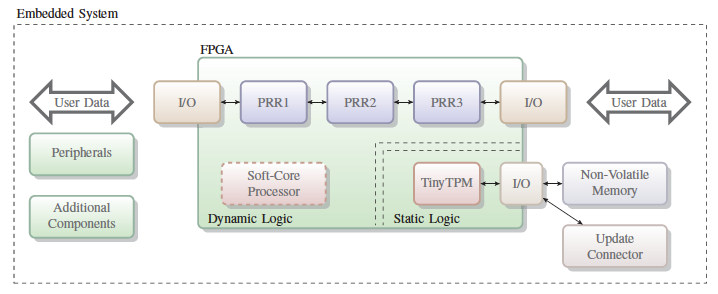
\includegraphics[scale=0.50]{images/tinyplatform.png}
\caption{Complete Architecture combined with TinyTPM}
\label{nome}
\end{figure}
TinyTPM bootstrap is simplificated respect canonical TPM requirements: a the initial bitstream is loaded into static part of the FPGA's logic, this initial state is called TinyTPM INIT STATE. Then, the FPGA is configured and the trusted module starts operation by executing a self test first. The integrity of the initially loaded bitstream is verified by comparison to reference value stored into NVM, thus building the root of trust. The NVM is accessible if and only if the initial bitstream is authentic. The result integrity measurement is then stored in $BCR_0$ for later reference. If this test goes well, the state of platform moves to INIT Dynamic Logic state, else the state return to TinyTPM INIT. [Mostrare figura e stati di TinyTPM]. In INIT Dynamic Logic State, all the partial bitstream are loaded. For each $PRR_n$ in the dynamic logic, the result of integrity measurement is stored in an individual $BCR_n$. Using monotonic counter this architecture can prevent replay attacks [inserire riferimento 8 di TinyTPM ed aggiungere qualche parola a riguardo].Once the static and the dynamic logic section are measured and configured, the embedded system is ready to accept command and work normally using the TinyTPM functionalities.  \\
In reference to the implementation during self authentication test during TPM boot, a set of commands is supplied to the ICAP interface to read the configuration of the FPGA. The output is grouped in 128 bit blocks and hashed using AES-based hash core. The result is then stored in $BCR_0$ for later reference\\. 
IP Core protection technique provided by TinyTPM architecture is widely described in the next section. \\
TinyTPM architecture is secure against an attacker able to monitor che communication between the authentic NVM and the TinyTPM residing n the FPGA because it is not able to gain any knowledge about the keys stored into NVM. 
% PARTE ATTESTAZIONE TINY TPM
Tiny TPM structure is presented before (inserire riferimento nel caso). Feller proposed an update protocol based on SKAP (Session Key Authorization Protocol) communication protocol designed by Chen [17TinyTPM]. This approach relies on public key cryptography to avoid both, TPM impersonaton and weak authorization data attacks. Before starting update process, a secure communication channel is established. 

The first step is an attestation of the platform request by the update server, TinyTPM response consist in a digitally signed set of BCR values to authenticate both itself and the system. After attestation, the update can be done. Update Manager sends PRMs(Partial Reconfiguration Module) to embedded system, where the data sent is authenticated and decrypted by the corresponding engines of the TinyTPM. As explained before, TinyTPM structure relies only on AES primitive, so the AES-based hash engine is used for computing hash values of the updated data. The computed hash values are then stored into BCRs of TinyTPM. Remember that an update data is stored in the NVM before loading it into the dynamic logic section of the FPGA. \\
In reference to the implementation, \emph{TPM\_Quote} operation realizes trustworthy reporting of the system state and creates a digital signature of  the stored BCR values. For this reason, the HMAC for all BCR values is computed sequentially and sent to the update server. Then update server, after a proper checking,sends updated bitstream in blocks of 128 bit size, because of the same blocks size of the utilized HMAC function. The number of the blocks is reported to TinyTPM within the first block. Upon reception the bitstream block is passed to HMAC core and additionally stored into BRA. Along with the last bitstream block the HMAC mode is changed to finalize the computation. Its result is compared to the final block containing the HMAC result computed by the update server. After successfully checking the HMAC, the resulting values is extended into the BCR and the bitstream is configured via the internal configuration access port (ICAP). (Il tutto è anche criptato dall'update server e decriptato nel sistema utente sempre usando la stessa chiave ovviamente eh!) 

\paragraph{PUF-based Trusted Execution Enviroment} \label{par:TEE}
In \cite{areno2012securing} a PUF-based TEE realization is proposed. A key stored in secureROM is the initial root-of-trust, where secureROM is inside SoC. Code included into TEE must be present at manufacturing time. This restrinction limits extension in all applications. The aim of this solution is to allow flexibility and possibility of alteration of the TEE after the manufacturing process.
\begin{figure}
\centering
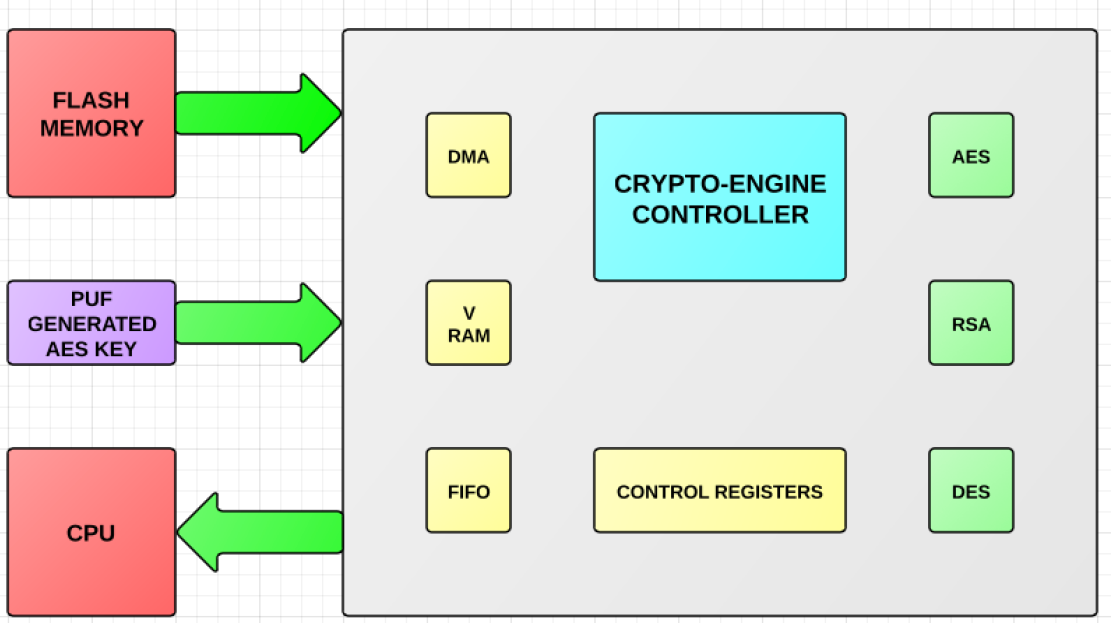
\includegraphics[scale=0.25]{images/teepuf.png}
\caption{PUF Supported Crypto-engine}
\label{fig:teeboot}
\end{figure}
TEE is typically stored in external non-volatile memory, if memory is not properly protected, it is subject to attack. Standard encryption helps to protect the TEE from this attacks. As explained before TTE cannot be customize for a specific implementation after manufacturing time. So in order to address this concern Areno \emph{et al} proposed the incorporation of a PUF inside Crypto-Engine of SoC. PUF will be used to generate secret AES Key giving additional security to TEE components. This approach also provides a means of modifying the TEE without requiring any changes to underlying hardware or software. \\
Any time an element of the TEE can be added/removed generating a new measurement encrypted using PUF key by crypto-engine. Because all measurements are encrypted by the PUF generated key, whose value is unknown to any entity and as such, any accidental or malicious alteration of this information is currently impossible. Figure \ref{fig:teeboot} shows modification into SoC architecture.  \\
This architecture is composed of:
\begin{itemize}
\item a controller which handles the flow of information through the engine,
\item a set of control registers often memory-mapped by CPU,
\item several cryptographic processor for specific operation such as AES, RSA or DES.
\end{itemize}
A small volatile RAM stores key generated by PUF: this key should not be accessible by any external element to blocks of cryptographic calculation. \\
This implementation can be useful for boot process. During boot time memory stored into secureROM is loaded and executed. Using PUF-based key, the secureROM content can be decrypted. This would provide the location, size and measurement of the TEE on the flash device. So TEE can be loaded into system. After the validation the system can run performing its operations. \\
TEE expansion with the proposed architecture does not require any additional hardware components. The primary purpose in supporting such addition is based upon the need of entities such as corporate IT departments to have a presence on mobile devices without emparing the usability of the device. Moreover, most corporate environment requires a device to be completely re-flashed  with their own version of the operating system. An application scenario is proposed in  \cite{areno2012securing} where a new employer install trusted-application on its device and when he leaves the company TEE component on the device are removed permitting to personal employer device to continue its normal functionalities. \\
A non-detailed architecture implementation on Xilinx FPGA is described of in \cite{areno2012securing}.


 

\subsubsection{ARM TrustZone Technology}
ARM\textsuperscript\textregistered TrustZone\textsuperscript\textregistered is a system approach that guarantees security for a wide range of clients including server, tablets, wearable devices and enterprise systems. This technology is integrated into Cortex\textsuperscript\textregistered -A processor family and is extended throughout the system via AMBA\textsuperscript\textregistered -AXI bus to specific TrustZone System IPBlocks  \footnote{http://www.arm.com/products/processors/technologies/trustzone/index.php}. \\
TrustZone permits to establishing trust in ARM-based platforms. TPMs are designed as fixed-function devices with a predefined and specified feature set while TrustZone represented a much more flexible approach by leveraging the CPU as a freely programmable trusted platform module. To do that, ARM introduced a special CPU mode called \emph{secure mode} in addition to the \emph{regular normal mode}. The notions of a "secure world" and a "normal world" follows previuos definition \ref{par:TEE}. Indeed ARM TrustZone is ARM own TEE implementation. \\
The TrustZone allows a processor to run application either in secure or non-secure world. It divide the single core in two virtual cores, one for each world. Switching from non-secure world to secure world is made by a Monitor. The possibilieties of a normal world processor to enter the secure world are strongly limitate to guarantee the resilency of TrustZone. Indeed, all the instructions that allow are exception. The assembly \emph{smc (Secure Mode Call)} istruction offer this switching possibility. Another important hardware change is the addition of NS-bit, a 33rd bit added to each internal address and data element that labels it as belongin to either the secure or non secure world. Figure \ref{fig:trustzonearchitecture} shows a general TrustZone architeture scheme. \\
\begin{figure}
\centering
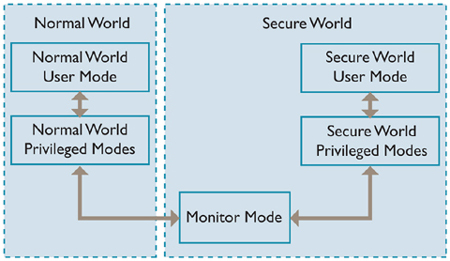
\includegraphics[scale=0.60]{images/trustzonearchitecture.jpg}
\caption{TrustZone Zone Structucture}
\label{fig:trustzonearchitecture}
\end{figure}
Inside a TrustZone-enabled processor there are two virtual MMU: one for every virtual processor. In this way, trusted area memory is logically detached from normal one. Thus there are two different set of andresses translation tables, making them indipendent. The tables uses a NS-field, this field is used by Secure Processor to verify that it belong to secure area. Normal processor ignores this field. However, Secure Processor can access to resources of both the worlds. Instead, caches supports both the worlds. \\
As presented before, ARM supplies the AMBA3 AXI TrustZone-enabled bus. This components manages the hardware logic to check that normal word cannot access to secret world resources. 
TrustZone implements three sets of interrupting vectors one for secure world: one for the non secure world and another one for monitor mode. \\
TrustZone, as other TEE systems, requires a Chain of Trust for its funcionalities. In order to create a Root of Trust, a key called \emph{PUK} is stored into an iROM, a processor-internal read-only memory. Such key is used to verify the integrity of the next booting phase, which will use the key to validate its successor, so the name Root of Trust. \\
A specific software have to run on TrustZone to exploit its specific hardware architecture. The Secure World has full control of hardware but secure process operating on it cannot directlu interact with non-trusted application. ARM released a standard API for the TrustZone in to simplify use for application developers. \\ 
Several trusted systems for mobile devices have been implemented leveraging ARM TrustZone techlogy, like Nokia's Onboard Credentials \cite{ekberg2008onboard}, \cite{kostiainen2009board} , Sierraware0s SierraTEE \footnote{http://www.sierraware.com}, this is used next. 
\begin{figure}
\centering
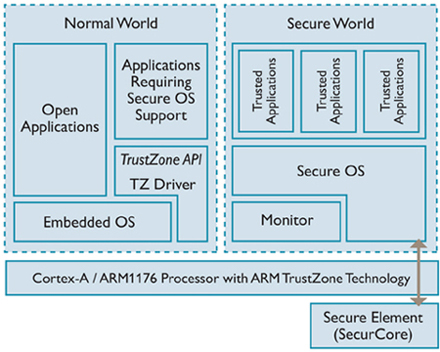
\includegraphics[scale=0.60]{images/trustzonesoftware.jpg}
\caption{TrustZone Software Architecture}
\label{fig:trustzonesoftware}
\end{figure}
\paragraph{SRAM PUF-based Root of Trust for ARM TrustZone}
Zhao \emph{et al} present a method to provide Root of Trust for ARM TrustZone using SRAM PUFs \cite{zhao2014providing}. Starting from TEE and TrustZone architecture shown before, \cite{zhao2014providing} implements a software entity, the building block. Building block provides the foundation for the root of trust: secure key storage and truly random source. Based on this building block, a root of trust is built to seal or unseal primitives for secure services running in the TEE. TPM is software-implemented.\\
Zhao proposal is based on this idea: a CPU with TrustZone security only provides an "isolated" execution environment, but not a \emph{trusted} one since it cannot attest to the user or an external verifier that the software running inside an untampered and trustworthy environment. \\
ARM does not specify explicitly the root of trust for TrustZone, so availability of an unique device key, as PUK key described before, is assumed. This key is accessible only inside the secure world of TrustZone and it is probably stored using Batter-back RAM or eFuse technologies, as already shown in \cite{barbareschi2014advancing}. In Zhao work this method is avoided and his own building block provides the foundation of a root of trust like:
\begin{itemize}
\item A primary seed extracted by a fuzzy extractor \ref{fuzzyextractor} form on-chip SRAM start-up values. This primary seed can be use to derive a device key,
\item A truly random seed extracted from the noise into on-chip SRAM start-up values. This random seed is used to build a RNG for the secure OS. 
\end{itemize} 
\begin{figure}
\centering
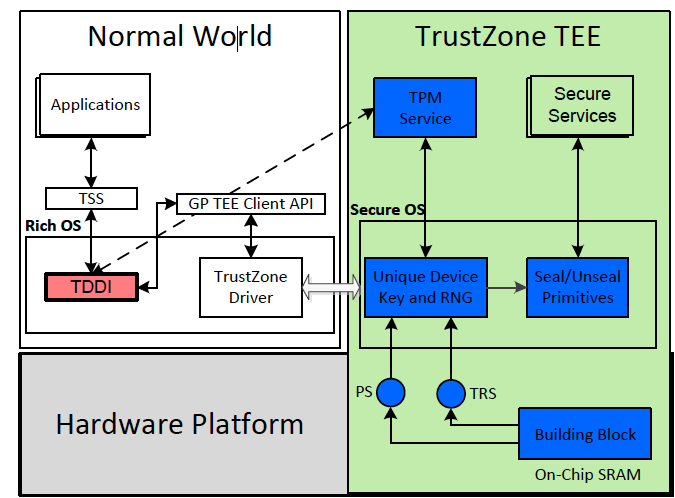
\includegraphics[scale=0.40]{images/zhaotee.png}
\caption{TrustZone Software Architecture}
\label{fig:zhaotee}
\end{figure}
This block also provides secure boot of the secure OS and secure services running inside the secure world of TrustZone. This feature is mandatory for a TrustZone. The building block is stored into secure on-chip SRAM achieving high security level, indeed this memory can resist against physical attacks on the SoC. The device key is used to provide seal and unseal primitives for secure services, which ensure that only specified secure service and platform can access user data. The seal/unseal primitives implicitly attest to the user the state of the platform and the secure service. Building Block operations consists in fuzzy extractor \emph{reproduce} functionality, it is described before in \ref{fuzzyextractor}. Building Block provides primary seed (PS) and truly random seed (TRS) as shown in figure \ref{fig:zhaotee}. \\
A developer can provide trusted computing functionalities with no need for additional security hardware resources so the build of root of trust is flexible and trustworthy. In order to facilitate the use of the TPM service, a kernel module called TDDI simulating a hardware TPM driver interface is provided in the normal world.
\begin{figure}
\centering
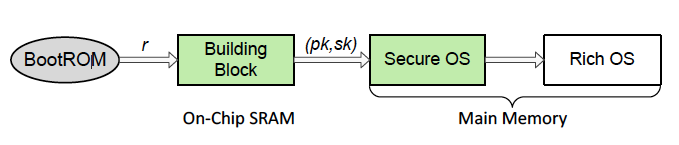
\includegraphics[scale=0.40]{images/zhaochainoftrust.png}
\caption{Building block-based Chain of Trust}
\label{fig:zhaochainoftrust}
\end{figure}
The simple seal and unseal primitives bind secure data with both the platform and the particual secure service throught cryptographic encryption or hashing. User data are encrypted with device key and this key is derived from the secure service. Only the device running a legitimate secure service with a right \emph{device key} can obtain the user data. Another situation is the offering of a secure service that permits to store sensitive data. \\
TPM service, which is realized in software, provides rich trusted computing functions for an OS. These functionalities can be used to bootstrap a trusted mobile OS and further help the normal world run in a trusted state. The TDDI helpt to use TPM services by simulating a TPM hardware driver interface. \\
In figure \ref{fig:zhaochainoftrust} is shown the chain of trust. A code designed for operation into secure world can be stored into insecure non-volatile storage so it is vulnerable to attacks from the normal world. However if a chain of trust is established from BootROM to the mobile OS, it is possible to protect integrity of the code running inside the secure world, such that mobile OS boot becomes trustworthy. \\
Analizing figure \ref{fig:zhaochainoftrust} when a device is powered up, ARM processor into secure mode performs code into BootROM. This code is immutable and defined at manufacturing time, so it is implicitly trusted. 
BootROM first operation is to verify the integrity of Building Block, so the image of it is measured and using manufacturer public key is possibile to do it analyzing the signature. So, the BootROM reads the start-up value r of the SRAM on chip, inizialiging it and load the building block in it. If integrity check succeeds, BootROM transfer \emph{r value} to building block and it runs building block in on-chip SRAM. \\
The role of buidling block is already known: it produces PS and TRS and then derive a symmetric key and unique device pair (pk,sk) from PS. Using this key pair image of Secure OS is verified: if check is successful the building block loads the image into secure memory region, else the system start up is stopped. When secure OS starts up, it initialized the services contained in the image, including TPM.  Then it measures the image of normal OS and finally secure OS runs the normal OS. \\
A significant improvement that PUF-based key can achive into system is the \emph{key update}. \cite{zhao2014providing} proposes a key update protocol which the device owner can change his device key regularly. The protocol provides in its steps a communication between the device and the manufacturer, the latter selects another challenge from a set already predisposed during manufacturing. \\
At the end of protocol device receives new \emph{Helper Data H'} to generate new primary seed, Secure OS encrypted with new \emph{symmetric key k'} and a \emph{certificate} with standard measurement values of the building block and secure OS. A drawback of this protocol is the weakness against downgrading attacks: an adversary can roll back the device key to an old one by copying previous helper data and encrypted blob of secure OS. Authers solve this issue with a secure monocounter. \\
In \cite{zhao2014providing} an implementation is shown using Xilinx Zinq-7000 AP SoC with a 256 KB on-chip SRAM inizialized by BootROM when board is powerred on. SRAM PUF is made using Altera Cyclone II connected via  Universal Asynchronous Receiver/Transmitter (UART) build using General  Purpose I/O (GPIO). The normal world runs Linux OS with kernel version 3.8, while the secure world runs Open Virtualization SierraTEE \footnote{SierraTEE for ARM TrustZone provides a minimal secure kernel which can be run in parallel with a more fully featured high level OS as Linux, Android, BSD. It also provides driver for the Rich OS to communicate with the secure kernel}. All the implemented Trusted Computing Base (TCB) is \emph{small} with a size of 3.2K LOC. 



\section{Hardware IP Cores Remote Activation}
%Zhang, Maes, Algodone...qualcosa andrebbe scritto...etc...ci sono anche molte cose nei related iniziali. 

\end{document}
